\documentclass[ACS,STIX2COL]{WileyNJD-v2}

\usepackage{amsmath,amssymb,amsfonts}
\usepackage{graphicx}
\usepackage{textcomp}
\usepackage{array}
\usepackage{booktabs}
\usepackage{multirow}
\usepackage{ragged2e}
\usepackage{siunitx}
\usepackage{tabularx}

\graphicspath{{./}}
\articletype{}%

\raggedbottom

\begin{document}

\title{Peak Aligned Gaussian Process Regression Assisted Plasmonic Refractive Index Sensor}

\author[1]{Md. Tajmimul Islam Soumik}
\author[1]{Md. Aslam Mollah*}
\author[2,3]{Abdulkarem H. M. Almawgani}
\author[3,4]{Hussein S. Gumaih}
\author[5]{Nurul Halimatul Asmak Ismail}
\author[6]{Monir Abdullah}
\author[7]{Samer A.B Awwad}
\author[8]{Jacob Wekalao}

%\authormark{SOUMIK \textsc{et al}.}

\address[1]{\orgdiv{Department of Electronics and Telecommunication Engineering}, \orgname{Rajshahi University of Engineering \& Technology (RUET)}, \orgaddress{\city{Rajshahi}, \country{Bangladesh}}}
\address[2]{\orgdiv{Electrical Engineering Department, College of Engineering}, \orgname{Najran University}, \orgaddress{\city{Najran}, \country{Saudi Arabia}}}
\address[3]{\orgdiv{Science and Engineering Research Center}, \orgname{Najran University}, \orgaddress{\city{Najran}, \country{Saudi Arabia}}}
\address[4]{\orgdiv{Biological Department, College of Science and Arts}, \orgname{Najran University}, \orgaddress{\city{Najran}, \country{Saudi Arabia}}}
\address[5]{\orgdiv{Department of Computer Science and Information Technology, Applied College}, \orgname{Princess Nourah bint Abdulrahman University}, \orgaddress{P.O. Box 84428, \city{Riyadh 11671}, \country{Saudi Arabia}}}
\address[6]{\orgdiv{Department of Computer Science and Artificial Intelligence, College of Computing and Information Technology}, \orgname{University of Bisha}, \orgaddress{\city{Bisha 61922}, \country{Saudi Arabia}}}
\address[7]{\orgdiv{Deanship of Information Technology and E-Learning}, \orgname{Imam Mohammad Ibn Saud Islamic University (IMSIU)}, \orgaddress{\city{Riyadh 11432}, \country{Saudi Arabia}}}
\address[8]{\orgdiv{Department of Optics and Optical Engineering}, \orgname{University of Science and Technology of China}, \orgaddress{96 Jinzhai Road, \city{Hefei 230026}, \country{China}}}

\corres{*Corresponding author: Md. Aslam Mollah. \email{ruet10aslam@gmail.com}}

\abstract[Abstract]{This study presents a machine-learning-assisted TiO$_2$-Au-coated photonic crystal fiber surface plasmon resonance (PCF-SPR) sensor that combines elliptical air holes with a U-shaped sensing slot for refractive index (RI) measurement. The proposed sensor offers the highest wavelength sensitivity of \textbf{44,000~nm/RIU}, and the figure of merit of \textbf{\boldmath$1100$~RIU$^{-1}$}. Additionally, a preprocessing technique is introduced to improve the detection of the resonance position using Gaussian process regression (GPR). The proposed approach, termed peak-aligned GPR, aligns the resonance features before model training, enabling more accurate prediction of both the resonance position and confinement-loss spectra compared with conventional GPR. The predicted spectra agree closely with the simulated data, giving \textbf{\boldmath$R^2=0.99729$}. The proposed sensor therefore offers great potential in SPR based RI sensing}

\keywords{Gaussian process regression, photonic crystal fiber, refractive index sensor, surface plasmon resonance}

\maketitle

\section{Introduction}

Surface plasmon resonance (SPR) enables label-free optical detection by tracking the resonance change produced by refractive-index variation at a metal-dielectric boundary\cite{khatun2026ml}. Integrating this effect with a photonic crystal fiber (PCF) creates a compact sensing structure that can be used in biomedical, chemical, and environmental measurements. In a PCF-SPR sensor, the strength of interaction between the guided core mode and the surface plasmon polariton (SPP) mode depends strongly on the air-hole arrangement, the position of the sensing region, and the selected coating materials\cite{md2026smart,ahammed2026machine}.

Machine learning (ML) is increasingly being combined with PCF-SPR sensing to limit repeated finite element method (FEM) calculations and to estimate sensor responses more quickly. Khatun and Islam developed an ML-XAI-assisted PCF-SPR design that achieved $R^2>0.99$ for effective-RI prediction together with a wavelength sensitivity of 12,000~nm/RIU \cite{khatun2026ml}. Md Abu \textit{et al.} reported a dual-channel ML-assisted sensor with 32,000~nm/RIU sensitivity and $R^2=0.9771$ \cite{md2026smart}. Ahammed \textit{et al.} found that their ML prediction was about 82.88 times faster than the corresponding FEM calculation \cite{ahammed2026machine}. For brain-tissue sensing, Akter \textit{et al.} obtained an MAE of $8.47\times10^{-6}$ using explainable ML \cite{akter2026neuropcf}. Rana \textit{et al.} used a Kolmogorov-Arnold network for confinement-loss estimation and reported $R^2=0.9996$ \cite{rana2026ultralow}.

ML-supported PCF-SPR systems have also been explored for several application-oriented sensing tasks. Ahmed \textit{et al.} applied a stacking ensemble to dual-analyte detection and obtained $R^2=0.9769$ \cite{ahmed2026simultaneous}. Grina \textit{et al.} introduced an IoT-based glucose sensor in which an MLP predicted confinement loss with $R^2=0.9963$ \cite{grina2026iot}. Shibly \textit{et al.} used an ANN to identify kerosene adulteration and reported a classification accuracy of 84.95\% \cite{shibly2026dual}. Sobur \textit{et al.} employed GBR and XGBR models for cancer-cell-related prediction, achieving $R^2=0.9912$ for effective RI \cite{sobur2025machine}. SHAP-based XAI was used by Khatun and Islam to assess the influence of sensor parameters \cite{khatun2025design}, whereas Mim \textit{et al.} demonstrated accurate RI estimation with a random-forest model \cite{mim2025advanced}.

Related work has applied ML-assisted PCF sensors to medical, biochemical, and environmental detection. Ahmed \textit{et al.} used more than 40,000 samples for deep-learning-based water-pathogen detection \cite{ahmed2025waterpathogen}. Other studies reported ANN-based acetylcholine sensing \cite{yadav2025enhanced}, RNN-LSTM pregnancy-stage monitoring with $R^2=0.9510$ \cite{ahmed2025pregnancy}, and ANN-based confinement-loss prediction with an MSE of $3.5363\times10^{-6}$ \cite{hamzaoui2025machine}. Further applications include malaria detection \cite{abdullah2026machine}, SPR optimization \cite{kaziz2024optimizing}, cancer-cell sensing \cite{bepare2026highly}, Au-TiO$_2$ malaria biosensing \cite{tayef2025highly}, and MCF-7 breast-cancer-cell detection \cite{jamil2025gold}.

Despite recent progress, complex D-shaped, polished, and dual-core sensors can be difficult to fabricate. Many ML-based methods also require large datasets generated through repeated FEM simulations, which increases computational cost \cite{md2026smart}. Direct spectrum prediction is especially challenging because the resonance peak shifts with RI.

To address these issues, this work uses a TiO$_2$-Au-coated PCF-SPR sensor with elliptical air holes and a U-shaped sensing slot. The slot strengthens analyte interaction with the plasmonic region, while the elliptical holes improve modal coupling. FEM is used to calculate the main sensing parameters. A peak-aligned GPR method is then applied to learn the spectral shape after aligning the resonance peaks, giving more stable and accurate predictions with fewer training samples than direct GPR.
% Design and Method
\section{Sensor Design and Numerical Method}


\subsection{PCF Structure With Initial Design Parameters}

Fig.~\ref{fig:proposed_structure} shows the cross section of the proposed TiO$_2$-Au-coated PCF-SPR sensor. Five elliptical air holes are arranged around the core in a pentagonal pattern at the optimized radial distance $R=4.6~\mu\mathrm{m}$. One hole forms a U-shaped analyte channel, which brings the sample closer to the guided and plasmonic fields. The initial semi-major axis is $a=1.8~\mu\mathrm{m}$, while $b$, $R$, and the TiO$_2$ and Au thicknesses use their optimized values. TiO$_2$ improves metal adhesion and modal coupling, whereas Au provides the SPR-active surface. Changes in analyte RI shift the phase-matching condition and therefore the resonance wavelength over the RI range 1.33-1.44.
\begin{figure}[!t]
    \centering
    
    % 2D cross-sectional diagram
    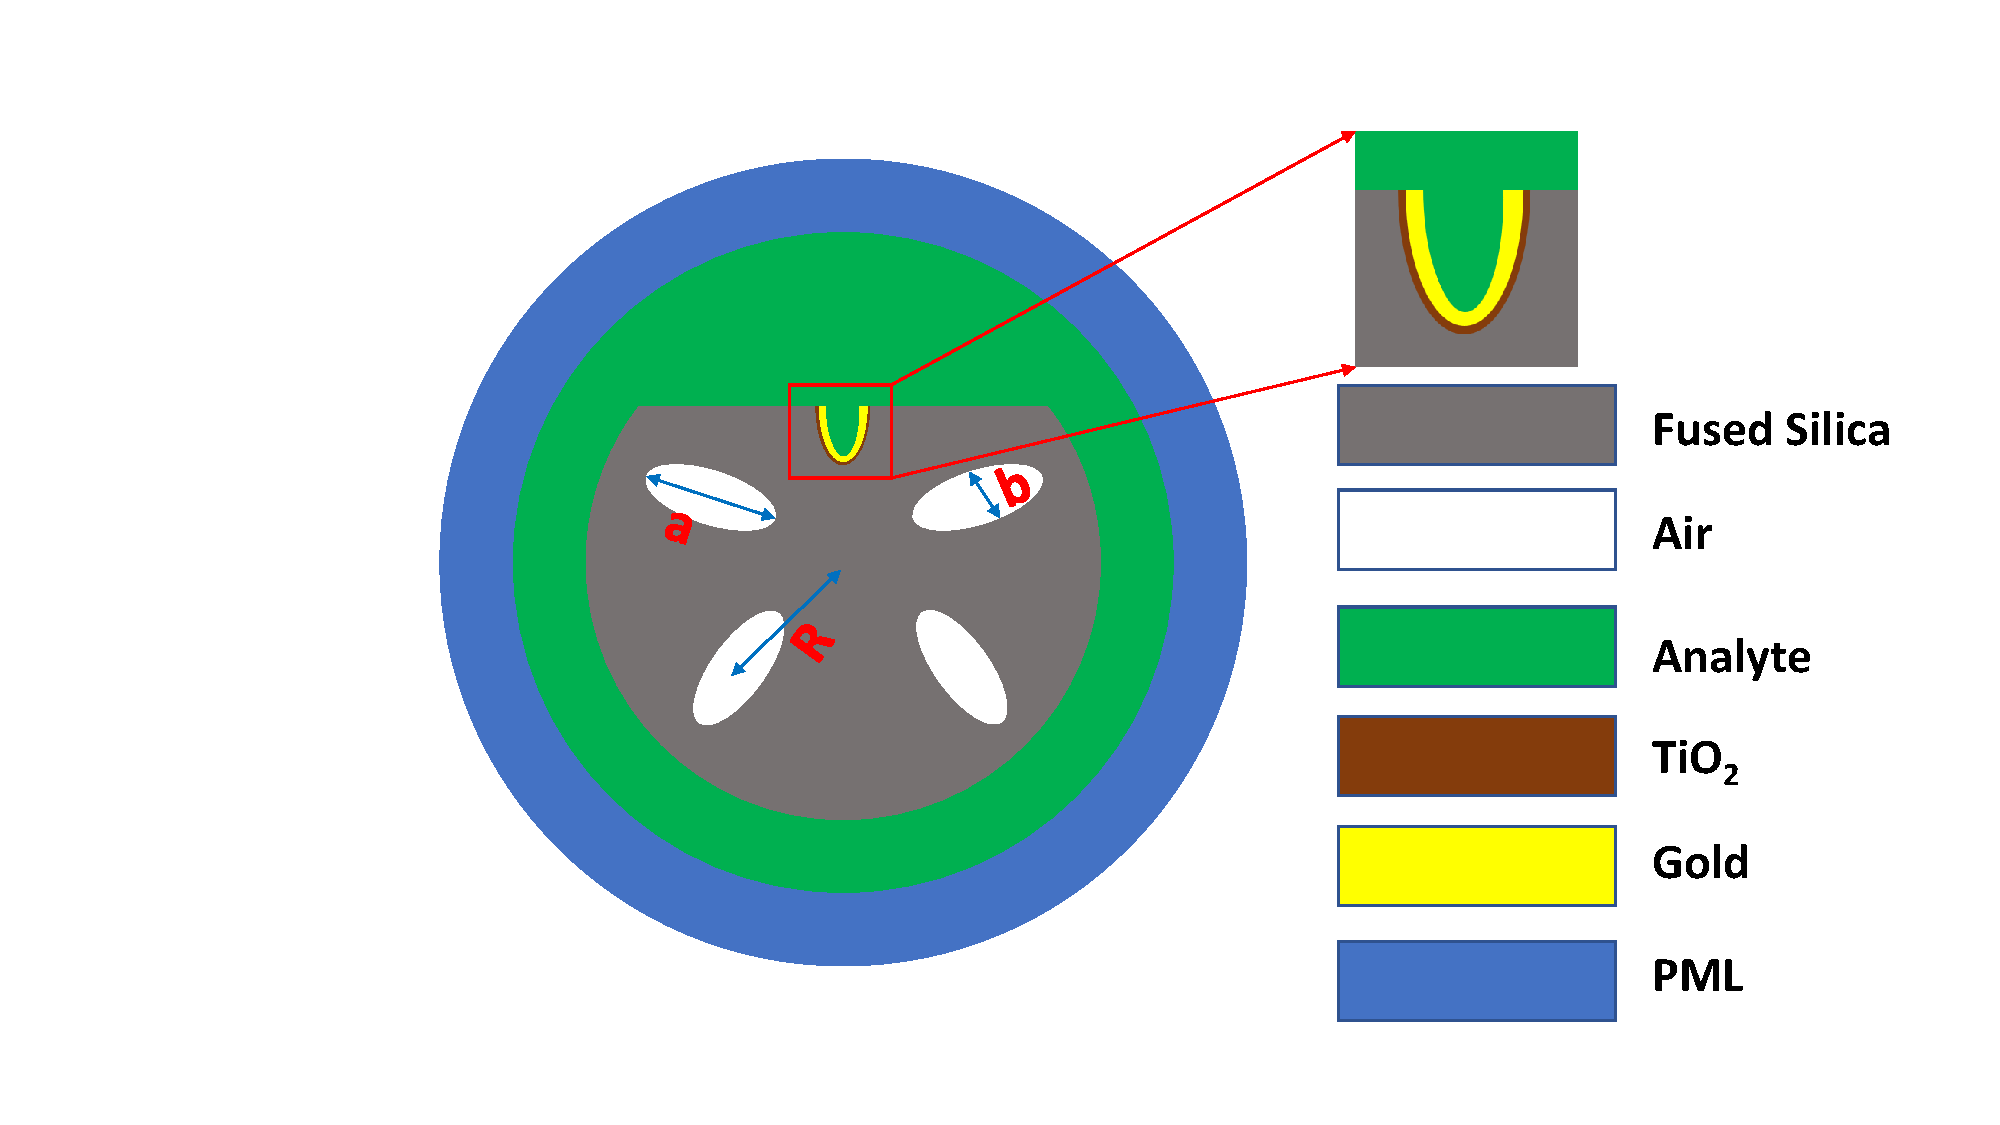
\includegraphics[width=\columnwidth]{2d_main_des_ellipse-Soumikpdf.pdf}
    
    
   \caption{Cross section of the proposed TiO$_2$-Au-coated U-slotted PCF-SPR geometry containing elliptical air holes.}
    \label{fig:proposed_structure}
\end{figure}

\subsection{Numerical Modelling}

The sensor is modelled in COMSOL Multiphysics using the finite element method (FEM). A circular perfectly matched layer (PML) absorbs outgoing fields and reduces boundary reflections. Eigenmode analysis is used to find the supported modes, while wavelength interrogation identifies the resonance for analyte RI values from 1.33 to 1.44.

Fused silica is used as the fiber material, and its wavelength-dependent RI is calculated from the Sellmeier equation \cite{ashrafian2025highly}:
\begin{equation}
n_{\mathrm{SiO_2}}(\lambda)=
\sqrt{
1+\frac{B_1\lambda^2}{\lambda^2-C_1}
+\frac{B_2\lambda^2}{\lambda^2-C_2}
+\frac{B_3\lambda^2}{\lambda^2-C_3}
}
\label{eq:sellmeier_silica}
\end{equation}
where $\lambda$ is in micrometers. The constants are $B_1=0.6961663$, $B_2=0.4079426$, $B_3=0.8974794$, $C_1=0.004679148~\mu\mathrm{m}^2$, $C_2=0.0135120631~\mu\mathrm{m}^2$, and $C_3=97.9340025~\mu\mathrm{m}^2$.

Gold is used as the plasmonic layer because of its stable SPR response. Its dielectric behavior is described by the Drude model \cite{zhang2025highlys}:
\begin{equation}
\varepsilon_{\mathrm{Au}}(\omega)
=
\varepsilon_{\infty}
-
\frac{\omega_p^2}{\omega(\omega+i\omega_c)},
\label{eq:au_drude}
\end{equation}
where $\omega$ is the angular frequency. The parameters are $\varepsilon_{\infty}=9.75$, $\omega_p=1.36\times10^{16}~\mathrm{rad\,s^{-1}}$, and $\omega_c=1.45\times10^{14}~\mathrm{rad\,s^{-1}}$.

A thin TiO$_2$ layer is placed between silica and Au to improve adhesion and strengthen guided-mode and plasmonic-mode coupling. Its RI is given by \cite{ashrafian2025highly}
\begin{equation}
n_{\mathrm{TiO_2}}(\lambda)=
\sqrt{
5.913+\frac{0.2441}{\lambda^2-0.0803}
}
\label{eq:tio2_ri}
\end{equation}
where $\lambda$ is in micrometers.

The confinement loss is calculated from the imaginary part of the modal effective RI \cite{zhang2025highly}:
\begin{equation}
\alpha_{\mathrm{loss}}(\mathrm{dB/cm})=
8.686\times\frac{2\pi}{\lambda}
\times \mathrm{Im}(n_{\mathrm{eff}})\times 10^4 .
\label{eq:confinement_loss}
\end{equation}
At resonance, strong coupling transfers power from the core mode to the SPP mode and creates a peak in the loss spectrum. The wavelength of this peak is taken as the resonance wavelength.
\subsection{Performance Indicating Parameters}

The sensor is evaluated using wavelength sensitivity, amplitude sensitivity, detection resolution, full width at half maximum (FWHM), and figure of merit (FOM). Wavelength sensitivity measures the resonance shift for a change in analyte RI \cite{zhang2025highlys}:
\begin{equation}
S_{\lambda}(\mathrm{nm/RIU})=
\frac{\Delta\lambda_{\mathrm{peak}}}{\Delta n_a}
\label{eq:wavelength_sensitivity}
\end{equation}
where $\Delta\lambda_{\mathrm{peak}}$ is the resonance shift and $\Delta n_a$ is the RI change.

Amplitude sensitivity describes the relative change in confinement loss with RI \cite{ashrafian2025highly}:
\begin{equation}
S_A(\lambda)\,[\mathrm{RIU}^{-1}]
=
-\frac{1}{\alpha(\lambda,n_a)}
\frac{\partial \alpha(\lambda,n_a)}{\partial n_a}
\label{eq:amplitude_sensitivity}
\end{equation}
where $\alpha(\lambda,n_a)$ is the confinement loss at wavelength $\lambda$ and analyte RI $n_a$.

Detection resolution represents the smallest measurable RI change \cite{ashrafian2025highly}:
\begin{equation}
R\,[\mathrm{RIU}]
=
\frac{\Delta n_a \times \Delta\lambda_{\min}}
{\Delta\lambda_{\mathrm{peak}}}
\label{eq:resolution}
\end{equation}
where the optical spectrum analyzer resolution is taken as $\Delta\lambda_{\min}=0.1$~nm.

The FOM is calculated from wavelength sensitivity and FWHM \cite{ashrafian2025highly}:
\begin{equation}
\mathrm{FOM}\,[\mathrm{RIU}^{-1}]
=
\frac{S_{\lambda}}{\mathrm{FWHM}}
\label{eq:fom}
\end{equation}
A narrower resonance gives a higher FOM and a clearer sensing response. All parameters are calculated over the RI range of 1.33-1.44.

\begin{figure}[!t]
    \centering
    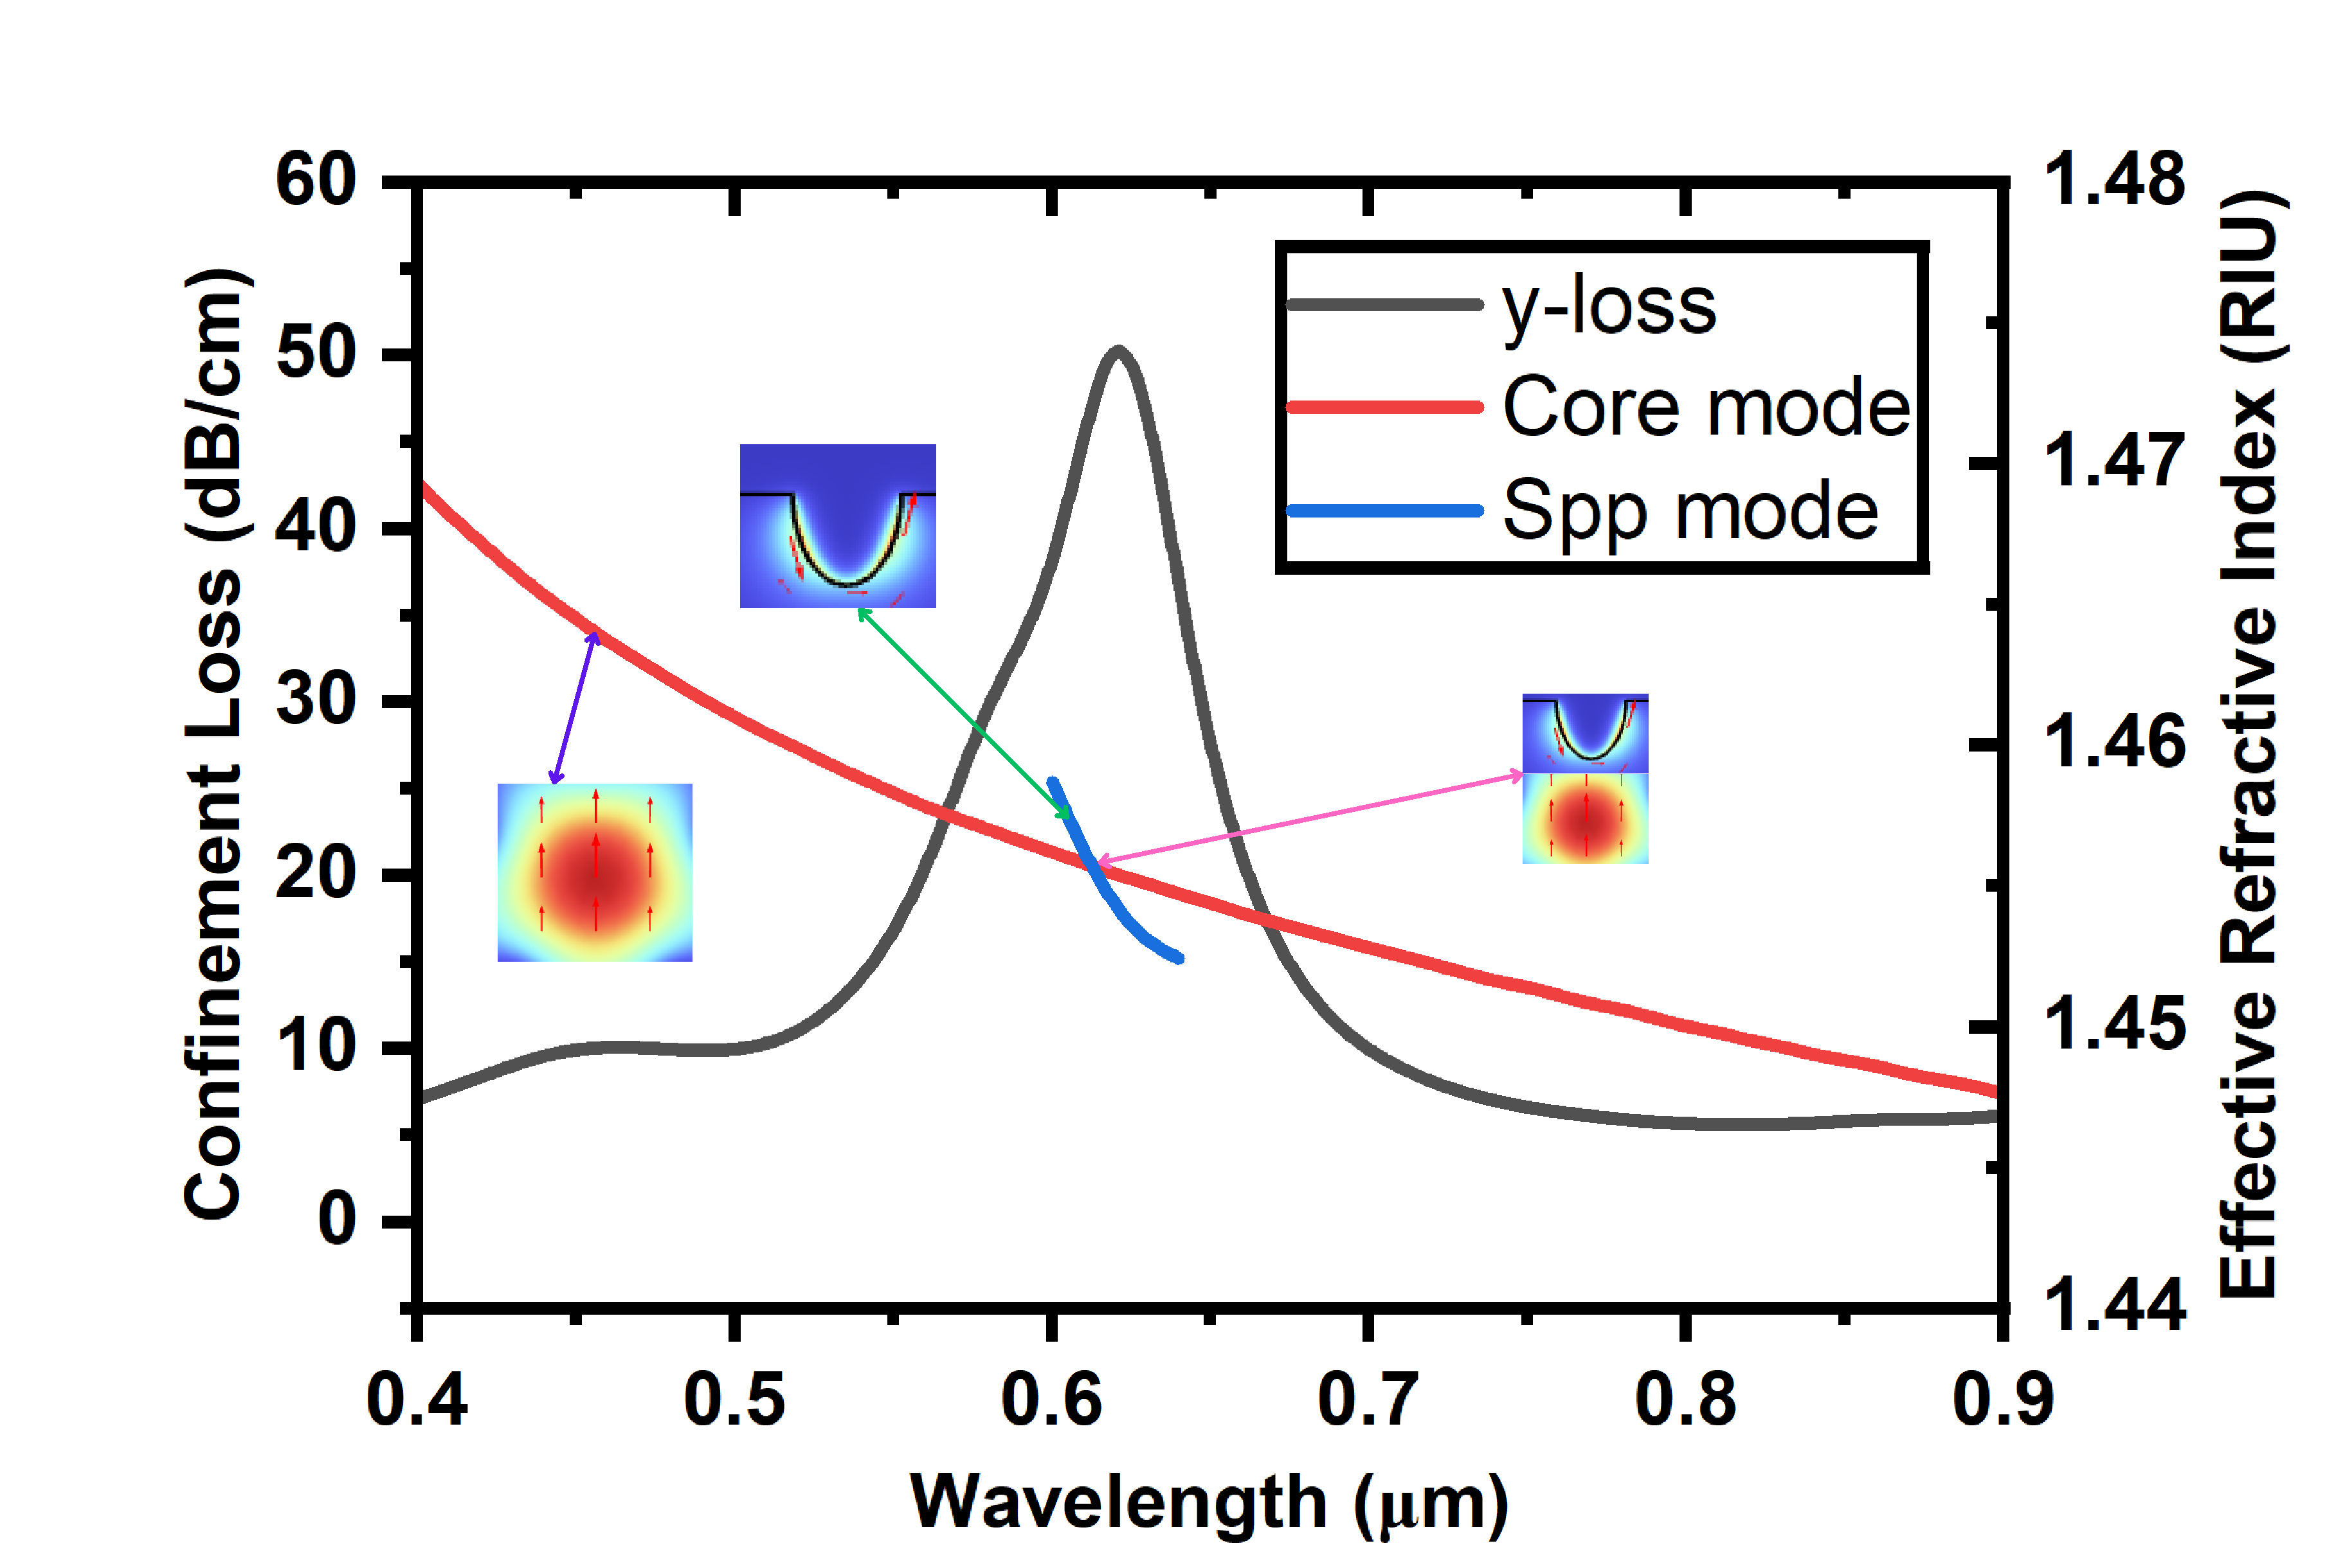
\includegraphics[
        width=0.75\columnwidth,
        trim={0 0 0 0},
        clip
    ]{phase-match.pdf}
    \caption{Phase-matching response of the proposed sensor at an analyte RI of 1.37.}
    \label{fig:phase_matching}
\end{figure}
\subsection{Resonance and Phase-Matching Behavior}

The phase-matching behavior is examined at $n_a=1.37$ in Fig.~\ref{fig:phase_matching}. As the wavelength changes, the effective index of the core-guided mode approaches that of the SPP mode supported by the Au interface. Their interaction becomes strongest near $0.61~\mu\mathrm{m}$, where a clear confinement-loss maximum appears. The field distributions in the insets also show that the optical field is concentrated around the U-shaped sensing region. Hence, the loss maximum is used to identify resonance, and the displacement of this maximum with RI forms the basis of the sensing process.
 
\begin{table*}[!t]
\centering
\caption{Calculated sensing metrics of the proposed TiO$_2$-Au-coated U-slotted elliptical-air-hole PCF-SPR sensor.}
\label{tab:sensing_performance}

\renewcommand{\arraystretch}{1.25}
\setlength{\tabcolsep}{4pt}
\scriptsize
\normalfont

\begin{tabular*}{\textwidth}{@{\extracolsep{\fill}}
c c c c c c c
@{}}

\toprule

\textbf{RI}
& \textbf{$\lambda_{\mathrm{peak}}$}
& \textbf{$S_{\lambda}$}
& \textbf{$S_A$}
& \textbf{FWHM}
& \textbf{FOM}
& \textbf{Resolution}
\\

&
\textbf{($\mu$m)}
& \textbf{(nm/RIU)}
& \textbf{(RIU$^{-1}$)}
& \textbf{($\mu$m)}
& \textbf{(RIU$^{-1}$)}
& \textbf{(RIU)}
\\

\midrule

1.33 & 0.56 & 1000  & -43.04   & 0.09 & 11.11   & $1.00\times10^{-4}$ \\
1.34 & 0.57 & 2000  & -53.86   & 0.09 & 22.22   & $5.00\times10^{-5}$ \\
1.35 & 0.59 & 1000  & -65.40   & 0.09 & 11.11   & $1.00\times10^{-4}$ \\
1.36 & 0.60 & 2000  & -94.93   & 0.09 & 22.22   & $5.00\times10^{-5}$ \\
1.37 & 0.62 & 2000  & -135.34  & 0.08 & 25.00   & $5.00\times10^{-5}$ \\
1.38 & 0.64 & 3000  & -213.36  & 0.07 & 42.86   & $3.33\times10^{-5}$ \\
1.39 & 0.67 & 4000  & -340.67  & 0.05 & 80.00   & $2.50\times10^{-5}$ \\
1.40 & 0.71 & 5000  & -480.80  & 0.04 & 125.00  & $2.00\times10^{-5}$ \\
1.41 & 0.76 & 7000  & -1167.11 & 0.04 & 175.00  & $1.43\times10^{-5}$ \\
1.42 & 0.83 & 12000 & -1074.38 & 0.03 & 400.00  & $8.33\times10^{-6}$ \\
1.43 & 0.95 & 44000 & -959.90  & 0.04 & 1100.00 & $2.27\times10^{-6}$ \\
1.44 & 1.39 & NA     & NA       & 0.15 & NA      & NA \\

\bottomrule

\end{tabular*}
\end{table*}

\section{Sensing Performance Analysis of the Proposed Sensor}
\begin{figure}[!t]
    \centering
    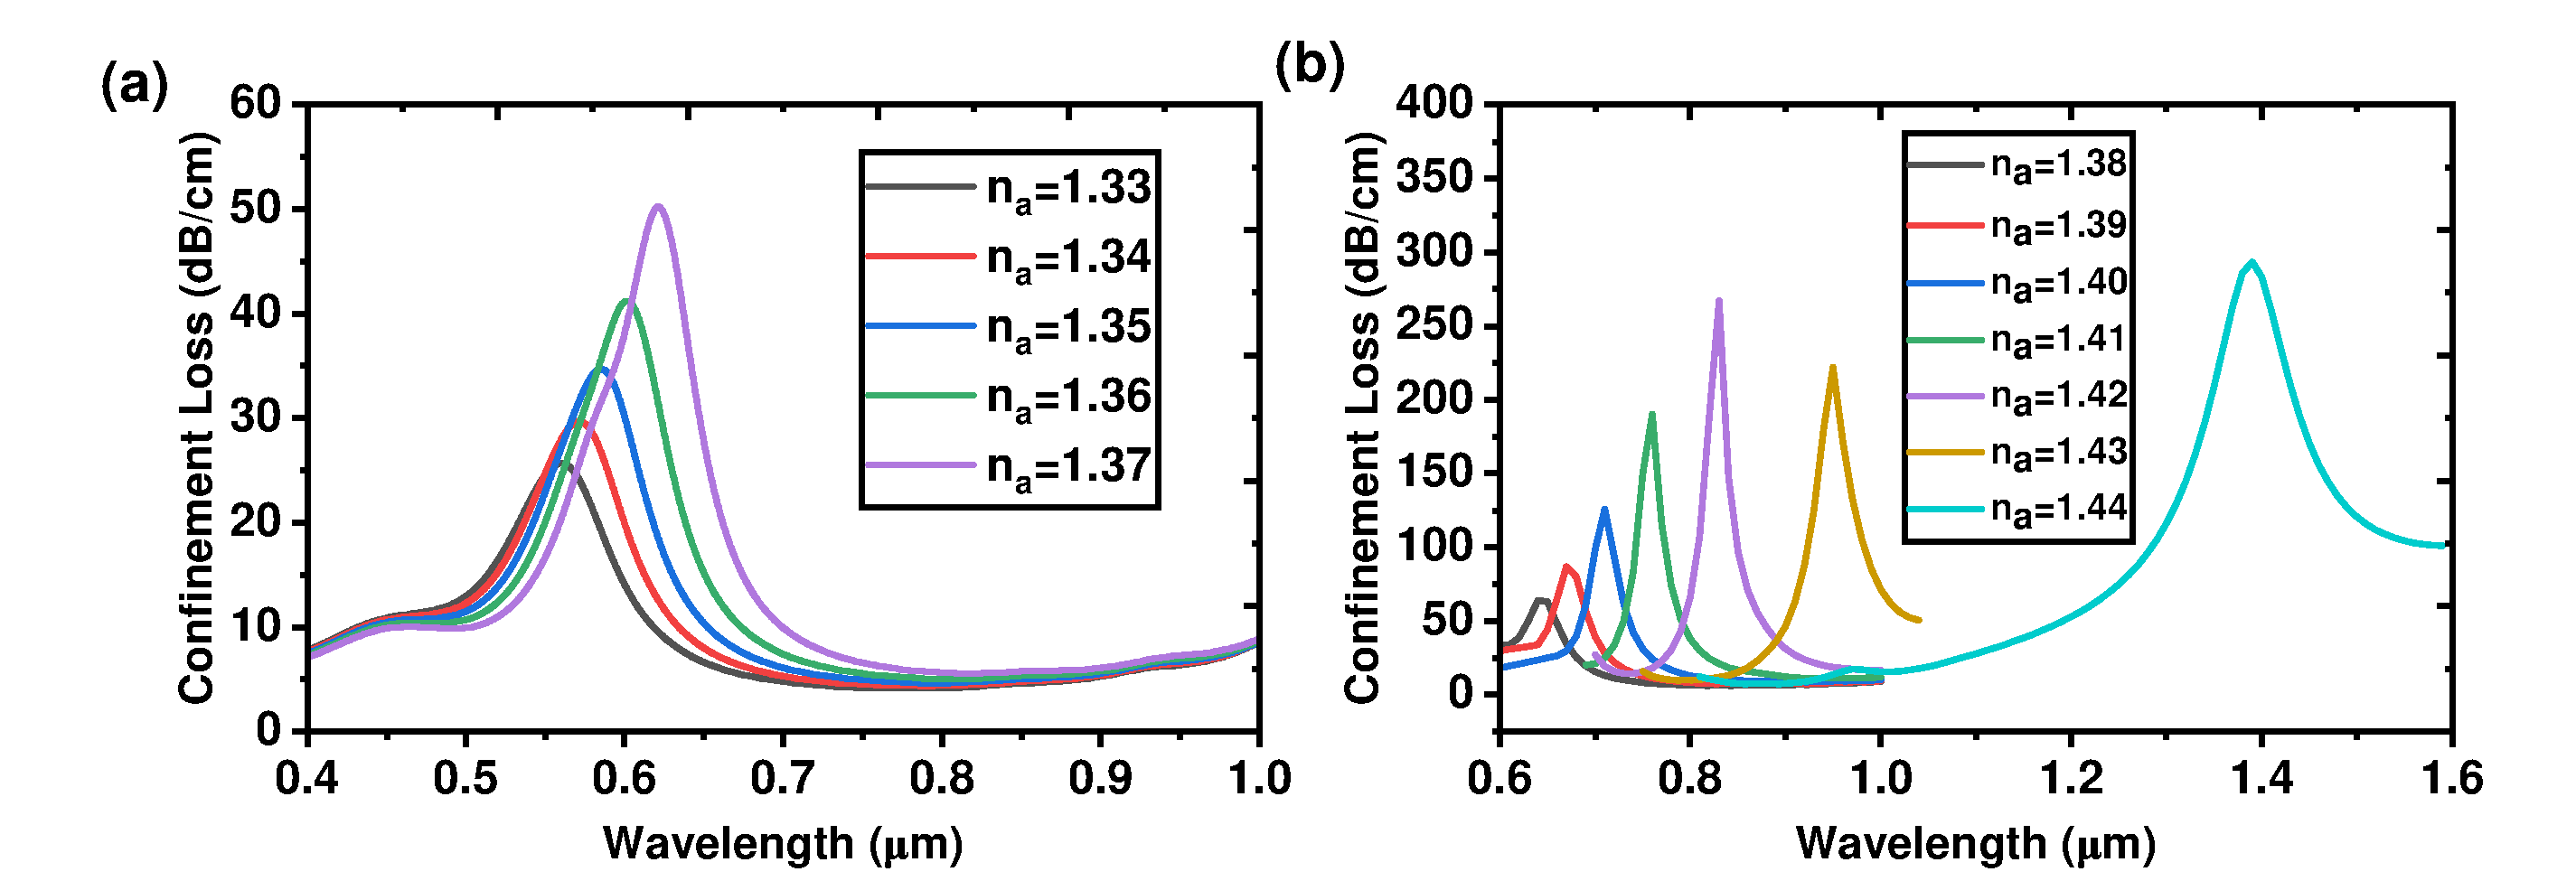
\includegraphics[width=\columnwidth]{cl-1.33-1.44_MS.pdf}
    \caption{Confinement-loss spectra of the proposed sensor for analyte RI values of (a) 1.33-1.37 and (b) 1.38-1.44.}
    \label{fig:cl_spectra}
\end{figure}
\subsection{Confinement Loss Response}
The confinement-loss spectra for RI values from 1.33 to 1.44 are shown in Fig.~\ref{fig:cl_spectra}. As the analyte RI increases, the resonance shifts to longer wavelengths because the core and SPP phase-matching condition changes. At higher RI values, the peak shift and loss increase, indicating stronger modal coupling. This clear red shift enables accurate detection of surrounding RI changes.




\subsection{Sensing Performance Analysis}

Table~\ref{tab:sensing_performance} summarizes the results for RI values from 1.33 to 1.44. The resonance wavelength shifts from $0.56$ to $1.39~\mu\mathrm{m}$ as the RI increases. The wavelength sensitivity reaches 44,000~nm/RIU at RI = 1.43, while the maximum amplitude sensitivity is $-1167.11~\mathrm{RIU}^{-1}$ at RI = 1.41. The highest FOM is 1100~RIU$^{-1}$, and the best resolution is $2.27\times10^{-6}$~RIU, confirming strong RI discrimination.

\begin{figure}[!t]
    \centering
    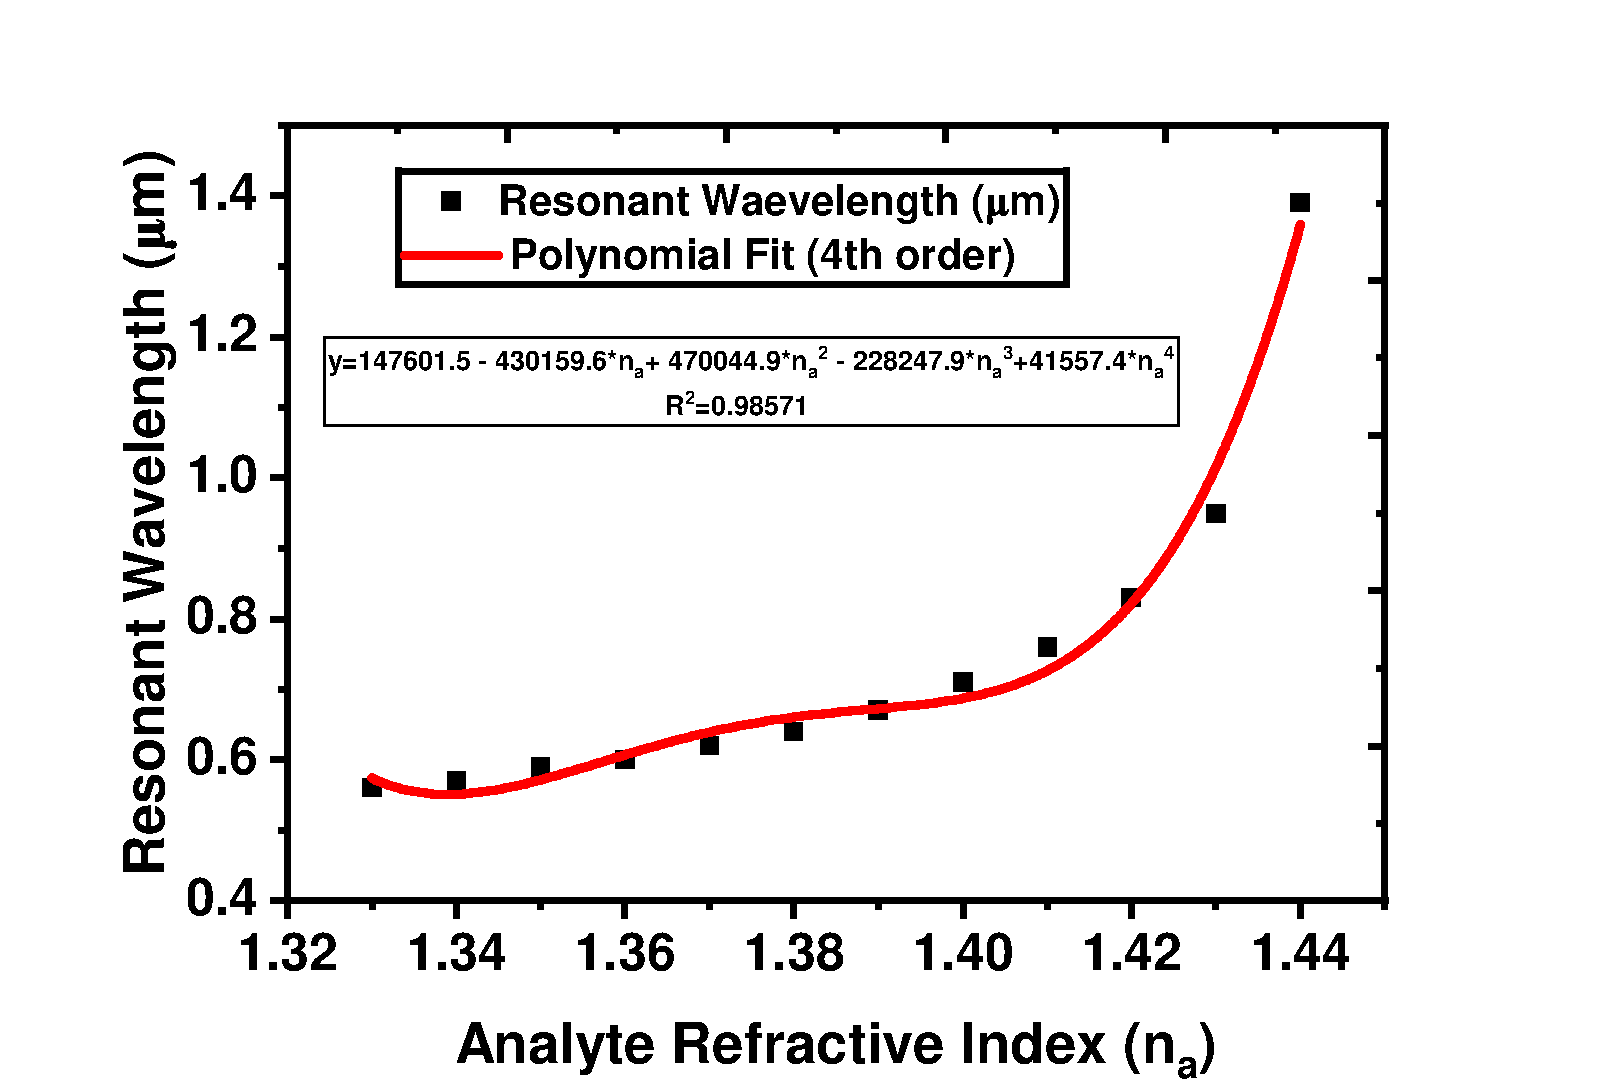
\includegraphics[width=0.75\columnwidth]{polynomial_soumik.pdf}
    \caption{Fourth-order polynomial calibration between analyte RI and resonance wavelength.}
    \label{fig:linearity_analysis}
\end{figure}


\subsection{Linearity Analysis}

Fig.~\ref{fig:linearity_analysis} shows the relationship between analyte RI and resonance wavelength. The resonance shifts to longer wavelengths as the RI increases from 1.33 to 1.44. Since the response becomes nonlinear above $n_a=1.42$, the calibration curve is fitted with a fourth-order polynomial:
\begin{equation}
\begin{aligned}
\lambda_{\mathrm{peak}} &= 147601.5 - 430159.6 n_a \\
&\quad {}+ 470044.9 n_a^2 - 228247.9 n_a^3 \\
&\quad {}+ 41557.4 n_a^4 .
\end{aligned}
\label{eq:poly_fit}
\end{equation}

Here, $n_a$ is the analyte RI and $\lambda_{\mathrm{peak}}$ is in $\mu$m. The fit gives $R^2=0.98571$, indicating good agreement with the simulated results.




\subsection{Cancer Cell Detection and Machine-Learning-Assisted Prediction}

The sensor response is also evaluated using RI values of normal and cancerous cervical and breast cells \cite{ashrafian2025highly}. As shown in Fig.~\ref{fig:cancer_cl_response}(a), the resonance shifts from $0.62~\mu\mathrm{m}$ for the normal cervical cell (RI = 1.3680) to $0.68~\mu\mathrm{m}$ for the HeLa cell (RI = 1.3920).

A similar shift is observed in Fig.~\ref{fig:cancer_cl_response}(b), where the resonance changes from $0.66~\mu\mathrm{m}$ for the normal breast cell to $0.71~\mu\mathrm{m}$ for the MCF-7 cell. These distinct peak positions allow the normal and cancerous samples to be identified from their confinement-loss spectra.

\begin{table*}[!t]
\centering
\caption{Sensing results for the normal and cancer-associated cell RI samples considered in this study.}
\label{tab:cancer_cell_detection}

\renewcommand{\arraystretch}{1.35}
\setlength{\tabcolsep}{4pt}
\scriptsize
\normalfont

\begin{tabular*}{\textwidth}{@{\extracolsep{\fill}}
l l c c c c c c c
@{}}

\toprule

\textbf{Cancer Type}
& \textbf{Cell Type}
& \textbf{RI}
& \textbf{$\lambda_{\mathrm{res}}$}
& \textbf{$S_{\lambda}$}
& \textbf{$S_A$}
& \textbf{FWHM}
& \textbf{FOM}
& \textbf{Resolution}
\\

&
&
& \textbf{($\mu$m)}
& \textbf{(nm/RIU)}
& \textbf{(RIU$^{-1}$)}
& \textbf{($\mu$m)}
& \textbf{(RIU$^{-1}$)}
& \textbf{(RIU)}
\\

\midrule

\multirow{2}{*}{Cervical cancer}
& Normal cervical cell
& 1.3680
& 0.62
& 2500
& -282.37
& 0.08
& 31.25
& $4.0\times10^{-5}$ \\

& HeLa cervical cancer cell
& 1.3920
& 0.68
& NA
& NA
& 0.04
& NA
& NA \\

\midrule

\multirow{2}{*}{Breast cancer}
& Normal breast cell
& 1.3850
& 0.66
& 3125
& -400.41
& 0.05
& 62.50
& $3.2\times10^{-5}$ \\

& MCF-7 breast cancer cell
& 1.4010
& 0.71
& NA
& NA
& 0.04
& NA
& NA \\

\bottomrule

\end{tabular*}
\end{table*}
\begin{figure}[!t]
    \centering
    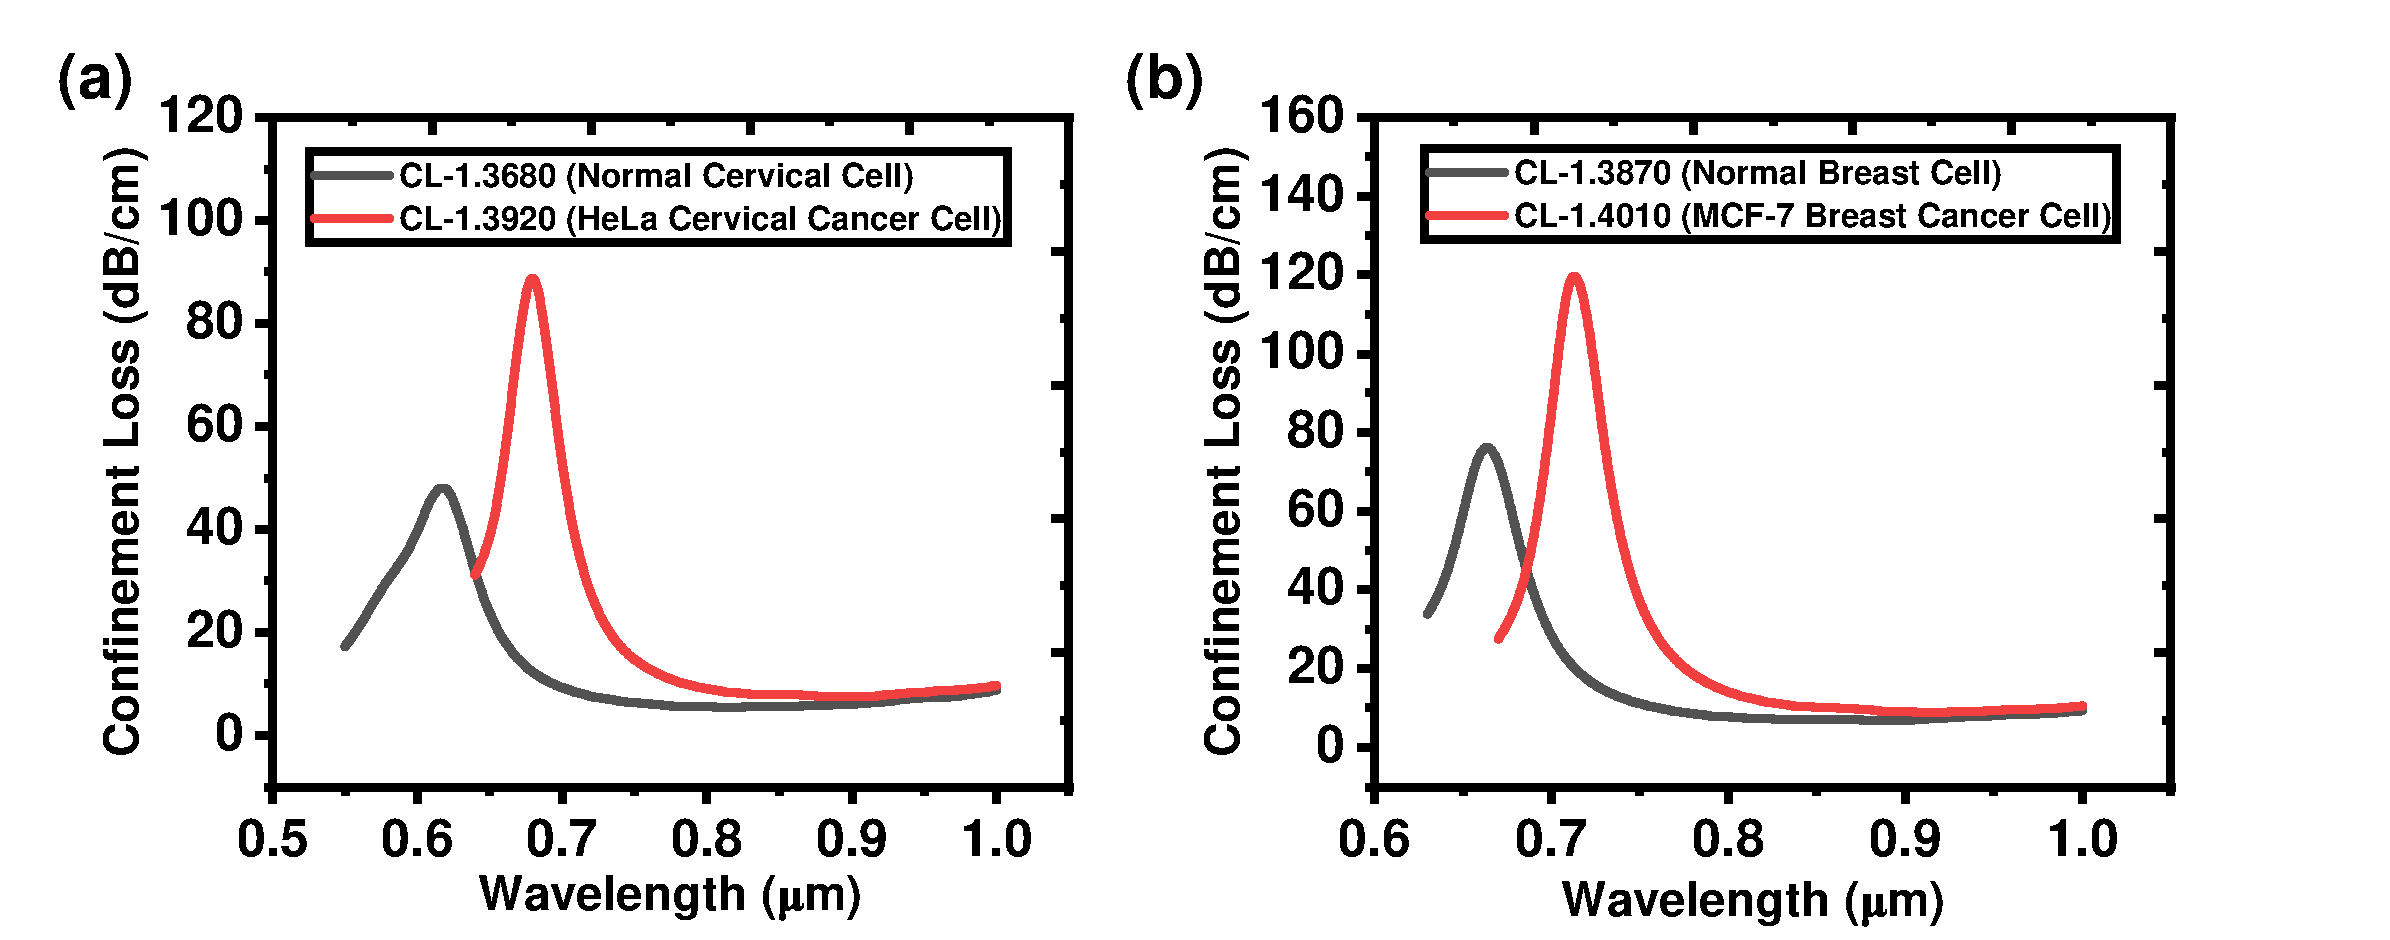
\includegraphics[width=\columnwidth]{cervical_breast.pdf}
    \caption{Confinement-loss comparison for (a) normal cervical and HeLa cells and (b) normal breast and MCF-7 cells.}
    \label{fig:cancer_cl_response}
\end{figure}
Table~\ref{tab:cancer_cell_detection} summarizes the sensing results. For the cervical-cell pair, the wavelength sensitivity, amplitude sensitivity, FOM, and resolution are 2500~nm/RIU, $-282.37$~RIU$^{-1}$, 31.25~RIU$^{-1}$, and $4.0\times10^{-5}$~RIU, respectively. For the breast-cell pair, these values are 3125~nm/RIU, $-400.41$~RIU$^{-1}$, 62.50~RIU$^{-1}$, and $3.2\times10^{-5}$~RIU. The different resonance peaks therefore allow normal and cancerous cells to be distinguished.

An ML model is used to predict the spectra without repeating the full-wave simulation for each RI. Confinement-loss spectra from RI = 1.33 to 1.42 are used for training, where $n_a$ is the input and $\alpha(\lambda,n_a)$ is the target. The cancer-cell RI values are reserved for testing.

Gaussian process regression (GPR) is selected because it performs well with small datasets and smooth nonlinear responses. The model uses scikit-learn's \texttt{GaussianProcessRegressor} with standardized inputs, normalized outputs, an RBF kernel, and a white-noise term \cite{pedregosa2011scikit}. The unknown relationship is represented as a Gaussian process: \cite{rasmussen2006gaussian},

\begin{equation}
f(n_a)\sim \mathcal{GP}\left(m(n_a),k(n_a,n_a')\right),
\label{eq:gpr_prior}
\end{equation}

where $m(n_a)$ represents the mean function and $k(n_a,n_a')$ is the covariance function. A squared-exponential kernel is adopted here to model the smooth dependence of the spectrum on RI \cite{rasmussen2006gaussian},

\begin{equation}
k(n_a,n_a')=\sigma_f^2\exp\left[-\frac{(n_a-n_a')^2}{2l^2}\right]+\sigma_n^2\delta_{n_a n_a'},
\label{eq:gpr_kernel}
\end{equation}

Here, $\sigma_f^2$ is the signal variance, $l$ is the kernel length scale, $\sigma_n^2$ represents the noise variance, and $\delta_{n_a n_a'}$ is the Kronecker delta.

Direct GPR must learn both the shifting peak position and the spectral shape, which is difficult with limited training data.

To make learning easier, each spectrum is shifted so that its resonance peak is centered at zero wavelength offset and then normalized by its peak loss. The peak wavelength and amplitude are calculated as

\begin{equation}
\begin{split}
\lambda_p(n_a) &= \operatorname*{arg\,max}_{\lambda}
\alpha(\lambda,n_a),\\
A_p(n_a) &= \max_{\lambda}\alpha(\lambda,n_a).
\end{split}
\label{eq:peak_extract}
\end{equation}

The aligned coordinate and normalized loss are then defined by

\begin{equation}
\tilde{\lambda}=\lambda-\lambda_p(n_a), \qquad
\tilde{\alpha}(\tilde{\lambda},n_a)=\frac{\alpha(\lambda,n_a)}{A_p(n_a)}.
\label{eq:peak_align}
\end{equation}

This preprocessing separates three quantities that would otherwise vary together: resonance position, resonance height, and spectral shape. Two multi-output GPR models are trained. The first estimates $\lambda_p$ and $\log(A_p)$, while the second learns the normalized aligned curve. The original confinement-loss spectrum is reconstructed from these outputs using

\begin{equation}
\hat{\alpha}(\lambda,n_a)=\exp(\hat{z}_p)\,
\hat{s}\left(\lambda-\hat{\lambda}_p\right),
\label{eq:peak_restore}
\end{equation}

Here, $\hat{\lambda}_p$ is the predicted resonance wavelength, $\hat{z}_p=\log(\hat{A}_p)$ represents the logarithm of the predicted peak loss, and $\hat{s}$ is the normalized spectral shape. The alignment follows curve registration, where major features such as resonance peaks are shifted to a common position before comparison or prediction \cite{ramsay2005functional,ramsay1998curve,james2007curve,marron2015functional}.

\begin{figure}[!t]
    \centering
    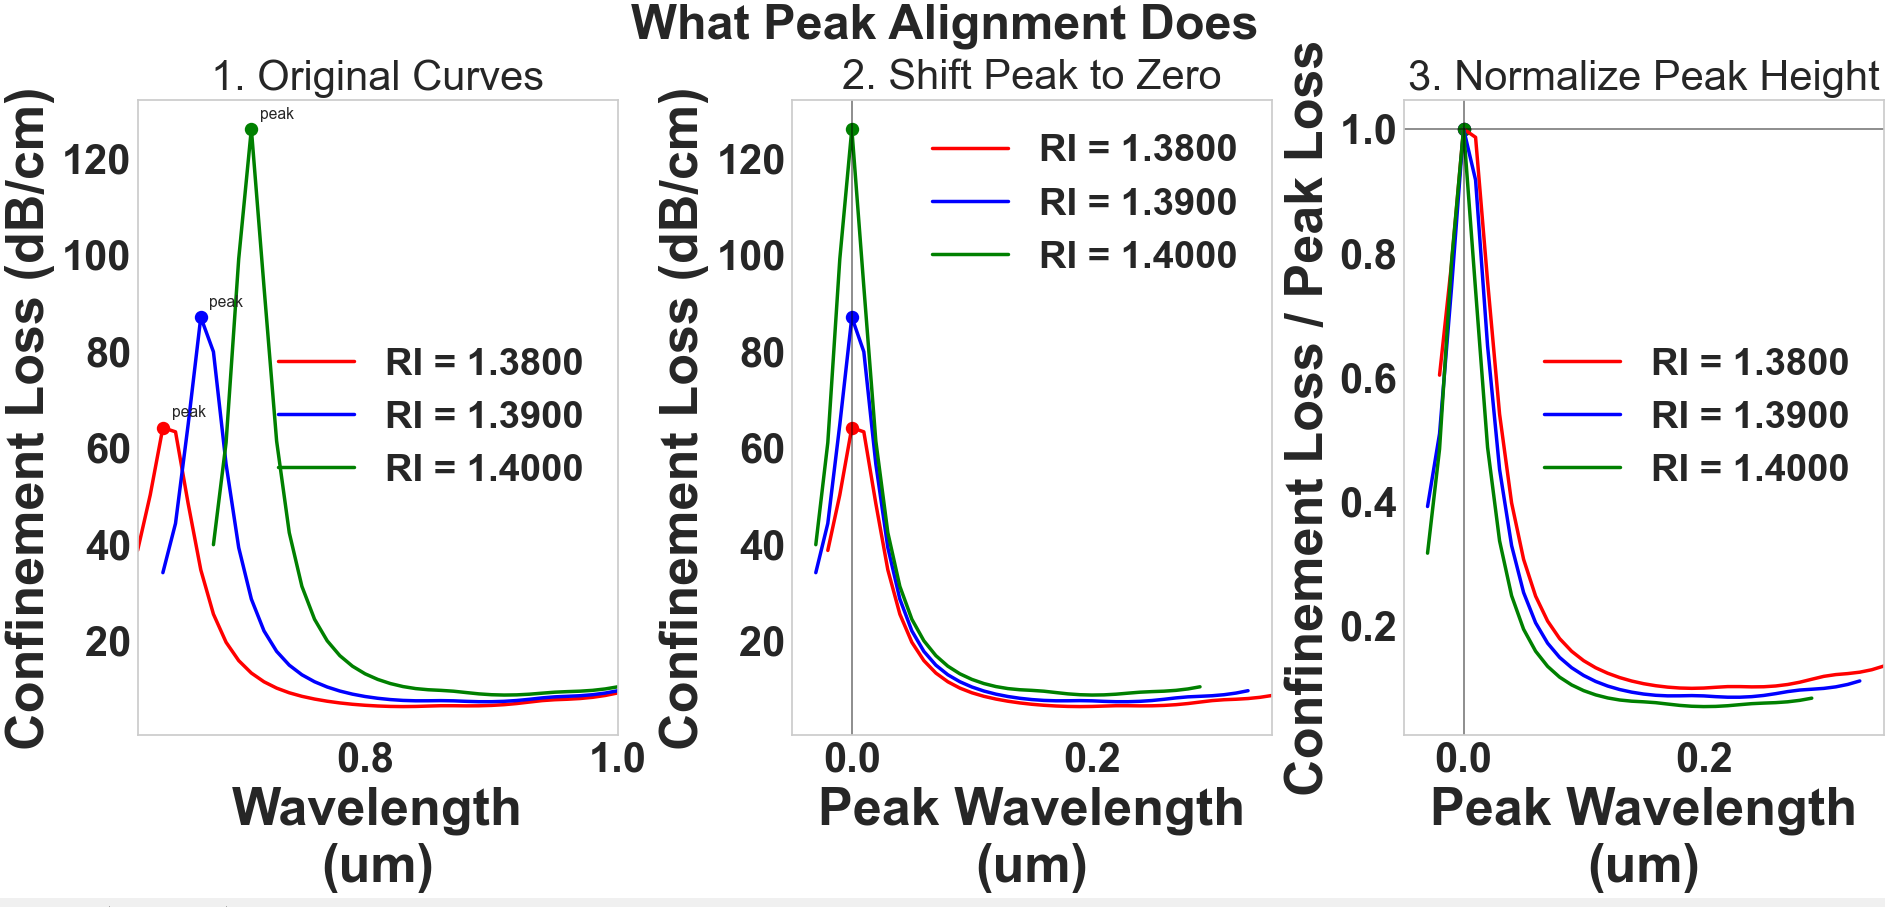
\includegraphics[width=\columnwidth]{peak-align.png}
    \caption{Preprocessing used for peak-aligned GPR: (a) original confinement-loss spectra, (b) spectra shifted to a common peak position, and (c) peak-normalized aligned spectra.}
    \label{fig:ml_peak_alignment}
\end{figure}

The three stages of spectral preprocessing are illustrated in Fig.~\ref{fig:ml_peak_alignment}. After the resonance peaks are moved to the same wavelength offset, each curve is scaled by its own peak loss. This removes most of the translation and amplitude variation from the shape-learning problem.

\begin{table}[!t]
\centering
\caption{Prediction accuracy obtained with the peak-aligned GPR model.}
\label{tab:gpr_testing_performance}

\renewcommand{\arraystretch}{1.25}
\setlength{\tabcolsep}{8pt}
\scriptsize
\normalfont

\begin{tabular}{l c c c}
\toprule
\textbf{Model} & \textbf{$R^2$} & \textbf{MAE} & \textbf{RMSE} \\
\midrule
Direct GPR 
& 0.95919
& 1.65687
& 3.68435 \\
\midrule
Peak-aligned GPR
& 0.99729
& 0.43319
& 0.94865 \\
\bottomrule
\end{tabular}
\end{table}

\begin{figure}[!t]
    \centering
    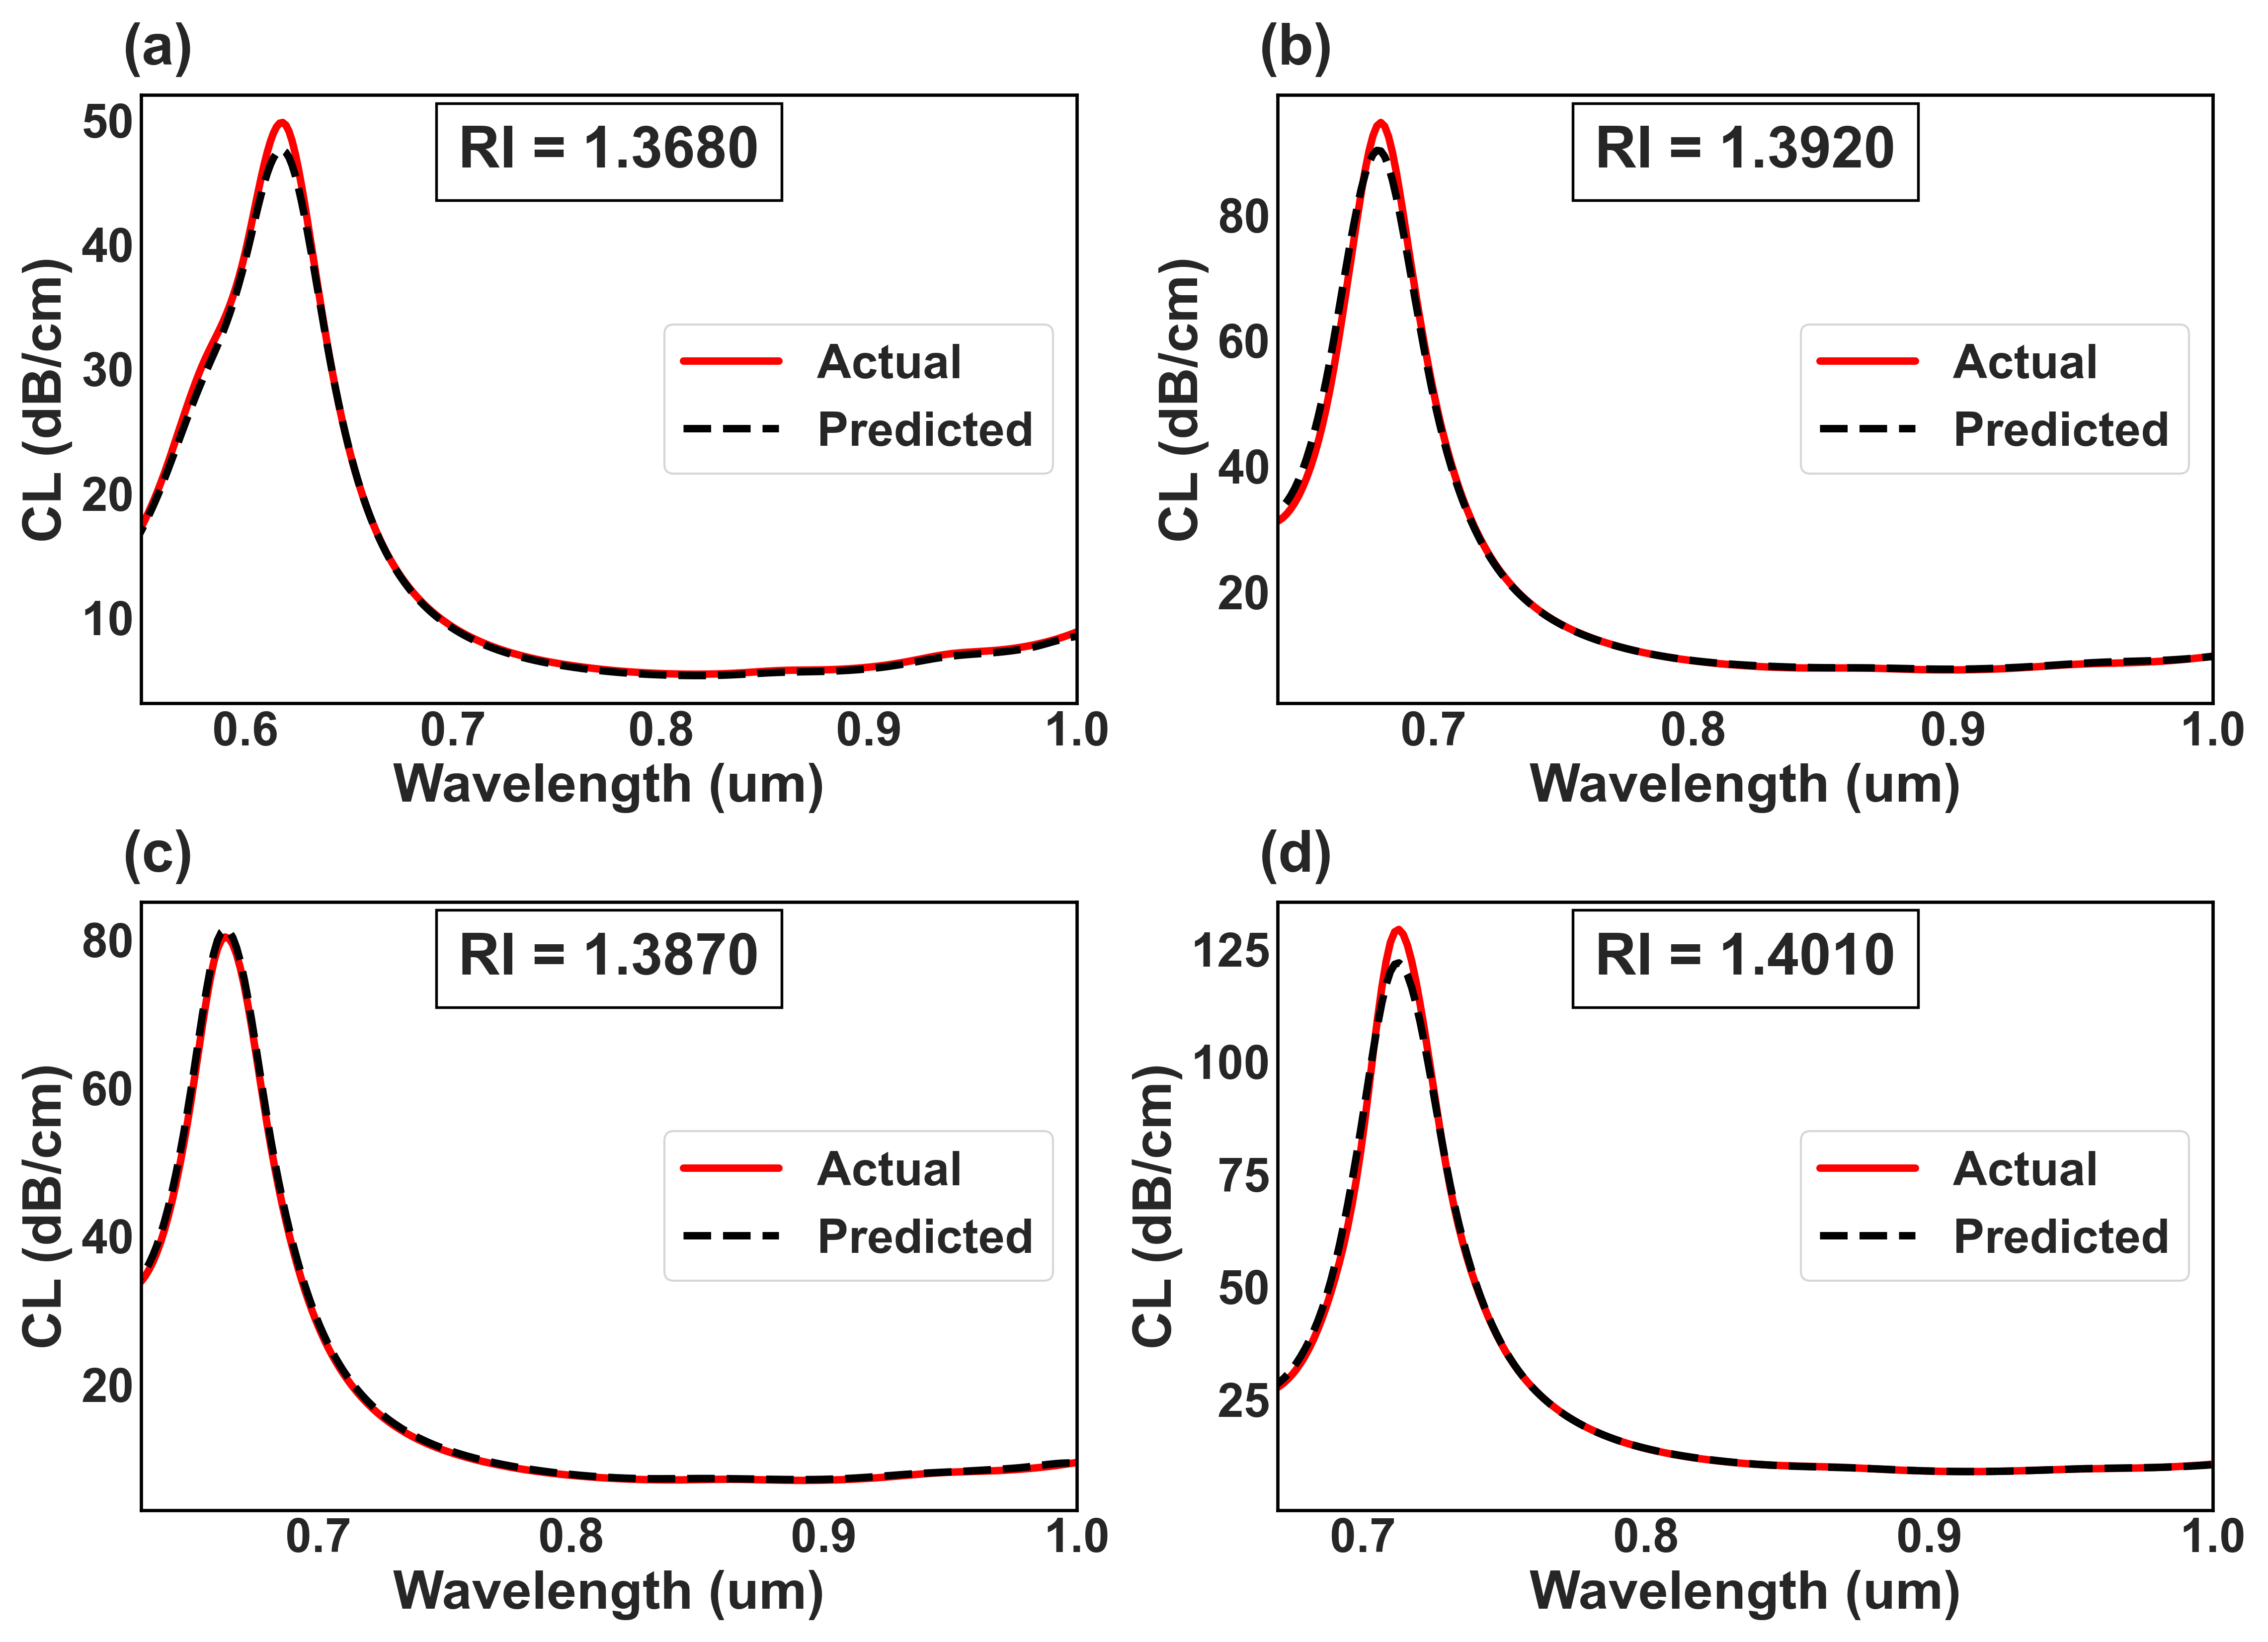
\includegraphics[width=\columnwidth]{option2_prediction_final.png}
    \caption{FEM and peak-aligned GPR confinement-loss spectra for the held-out cancer-cell RI samples.}
    \label{fig:ml_peak_aligned_gpr_prediction}
\end{figure}

Table~\ref{tab:gpr_testing_performance} compares the two models. Direct GPR achieved $R^2=0.95919$, MAE = 1.65687, and RMSE = 3.68435. The peak-aligned model improved these results to $R^2=0.99729$, MAE = 0.43319, and RMSE = 0.94865, showing much closer agreement with the FEM spectra.

\begin{table*}[!t]
\centering
\caption{FEM and GPR estimates of resonance wavelength and peak loss for the selected cancer-cell RI samples.}
\label{tab:actual_predicted_peak}
\renewcommand{\arraystretch}{1.25}
\setlength{\tabcolsep}{6pt}
\scriptsize

\begin{tabular*}{\textwidth}{@{\extracolsep{\fill}} l c c c c c @{}}
\toprule

\textbf{Cell Sample}
& \textbf{RI}
& \multicolumn{2}{c}{\textbf{Actual FEM Result}}
& \multicolumn{2}{c}{\textbf{Peak-Aligned GPR}} \\

\cmidrule(lr){3-4}
\cmidrule(lr){5-6}

&
& \textbf{$\lambda_p$ ($\mu$m)}
& \textbf{Peak Loss (dB/cm)}
& \textbf{$\hat{\lambda}_p$ ($\mu$m)}
& \textbf{Peak Loss (dB/cm)} \\

\midrule

Normal cervical cell      
& 1.3680 & 0.62 & 49.45  & 0.62 & 47.29 \\

HeLa cervical cancer cell 
& 1.3920 & 0.68 & 94.67  & 0.68 & 90.05 \\

Normal breast cell        
& 1.3870 & 0.66 & 78.60  & 0.66 & 79.75 \\

MCF-7 breast cancer cell  
& 1.4010 & 0.71 & 126.95 & 0.71 & 120.33 \\

\bottomrule
\end{tabular*}
\end{table*}

% Comparison of FEM and GPR peak parameters is discussed after Table~\ref{tab:comparative_ml}.
\begin{table*}[!t]
\centering
\caption{Comparison of the proposed design with selected ML-assisted SPR sensors reported in the literature.}
\label{tab:comparative_ml}

\renewcommand{\arraystretch}{1.35}
\setlength{\tabcolsep}{3pt}
\scriptsize
\normalfont

\resizebox{\textwidth}{!}{
\begin{tabular}{l p{4.0cm} p{3.0cm} c c c}

\toprule

\textbf{Ref.}
& \textbf{Biosensor Type}
& \textbf{Model}
& \textbf{RI Range}
& \textbf{$R^2$}
& \textbf{Max WS}
\\

&
&
&
&
&
\textbf{(nm/RIU)}
\\

\midrule

\cite{ahmed2026simultaneous}
& Stacking-based ensemble ML-optimized PCF-SPR multi-analyte biosensor
& RFR-GBR-DTR stacking
& 1.15-1.41
& 0.9769
& 10,000 \\

\cite{sobur2025machine}
& ML-enhance SPR-based optical biosensor for cancer-cell detection
& GBR/XGBR
& 1.33-1.40
& 0.9912/0.9278
& 10,000 \\

\cite{khatun2026ml}
& ML-XAI-assisted PCF-SPR sensor for naringenin detection
& RF/GPR with XAI
& 1.3740-1.3862
& $>$0.99/$>$0.93
& 12,000 \\

\cite{md2026smart}
& ML-augmented dual-channel PCF-SPR biosensor
& RF-GB-XGBoost ensemble
& 1.33-1.45
& 0.9771
& 32,000 \\

\cite{yadav2025enhanced}
& D-shape PCF-SPR biosensor for acetylcholine detection
& ANN
& 1.33-1.42
& 0.944
& 34,442.96 \\

\textbf{Proposed Work}
& \textbf{TiO$_2$-Au-coated U-slotted elliptical-air-hole PCF-SPR sensor}
& \textbf{Peak-aligned GPR}
& \textbf{1.33-1.44}
& \textbf{0.99729}
& \textbf{44,000} \\

\bottomrule

\end{tabular}
}
\end{table*} 
Table~\ref{tab:actual_predicted_peak} compares the FEM and GPR peak results for the selected cancer-cell RI values. The predicted resonance wavelengths match the FEM values to the reported precision, while the peak losses remain close. This shows that the peak-aligned model can accurately estimate both resonance position and magnitude.

Fig.~\ref{fig:ml_peak_aligned_gpr_prediction} further shows that the predicted spectra preserve the correct peak locations and overall curve shapes. The model is therefore suitable for fast spectral prediction, while FEM remains the reference for physical validation.

\subsection{Performance Comparison with Existing ML-Assisted SPR Sensors}

Table~\ref{tab:comparative_ml} compares the proposed sensor with several recent ML-assisted SPR biosensors. Most reported works achieve maximum wavelength sensitivities between 10,000 and 34,442.96~nm/RIU, while the proposed design reaches 44,000~nm/RIU. The peak-aligned GPR model also provides a high prediction accuracy with an $R^2$ value of 0.99729 over the RI range of 1.33--1.44. Overall, the proposed sensor shows a strong combination of wide RI coverage, high sensitivity, and reliable ML-based prediction compared with the selected existing approaches.


\section{Parametric Optimization of the Proposed Sensor}

The geometric and coating parameters are optimized one at a time by varying $a$, $b$, $R$, and the TiO$_2$ and Au thicknesses while keeping the other values fixed. Their effects on resonance wavelength, confinement loss, wavelength sensitivity, and amplitude sensitivity are evaluated at RI = 1.38 and 1.39 using Fig.~\ref{fig:optimization_curves} and Table~\ref{tab:optimization_results}. The final values are selected from the best overall balance of these performance measures, not from wavelength sensitivity alone.
\begin{figure}[!t]
\centering

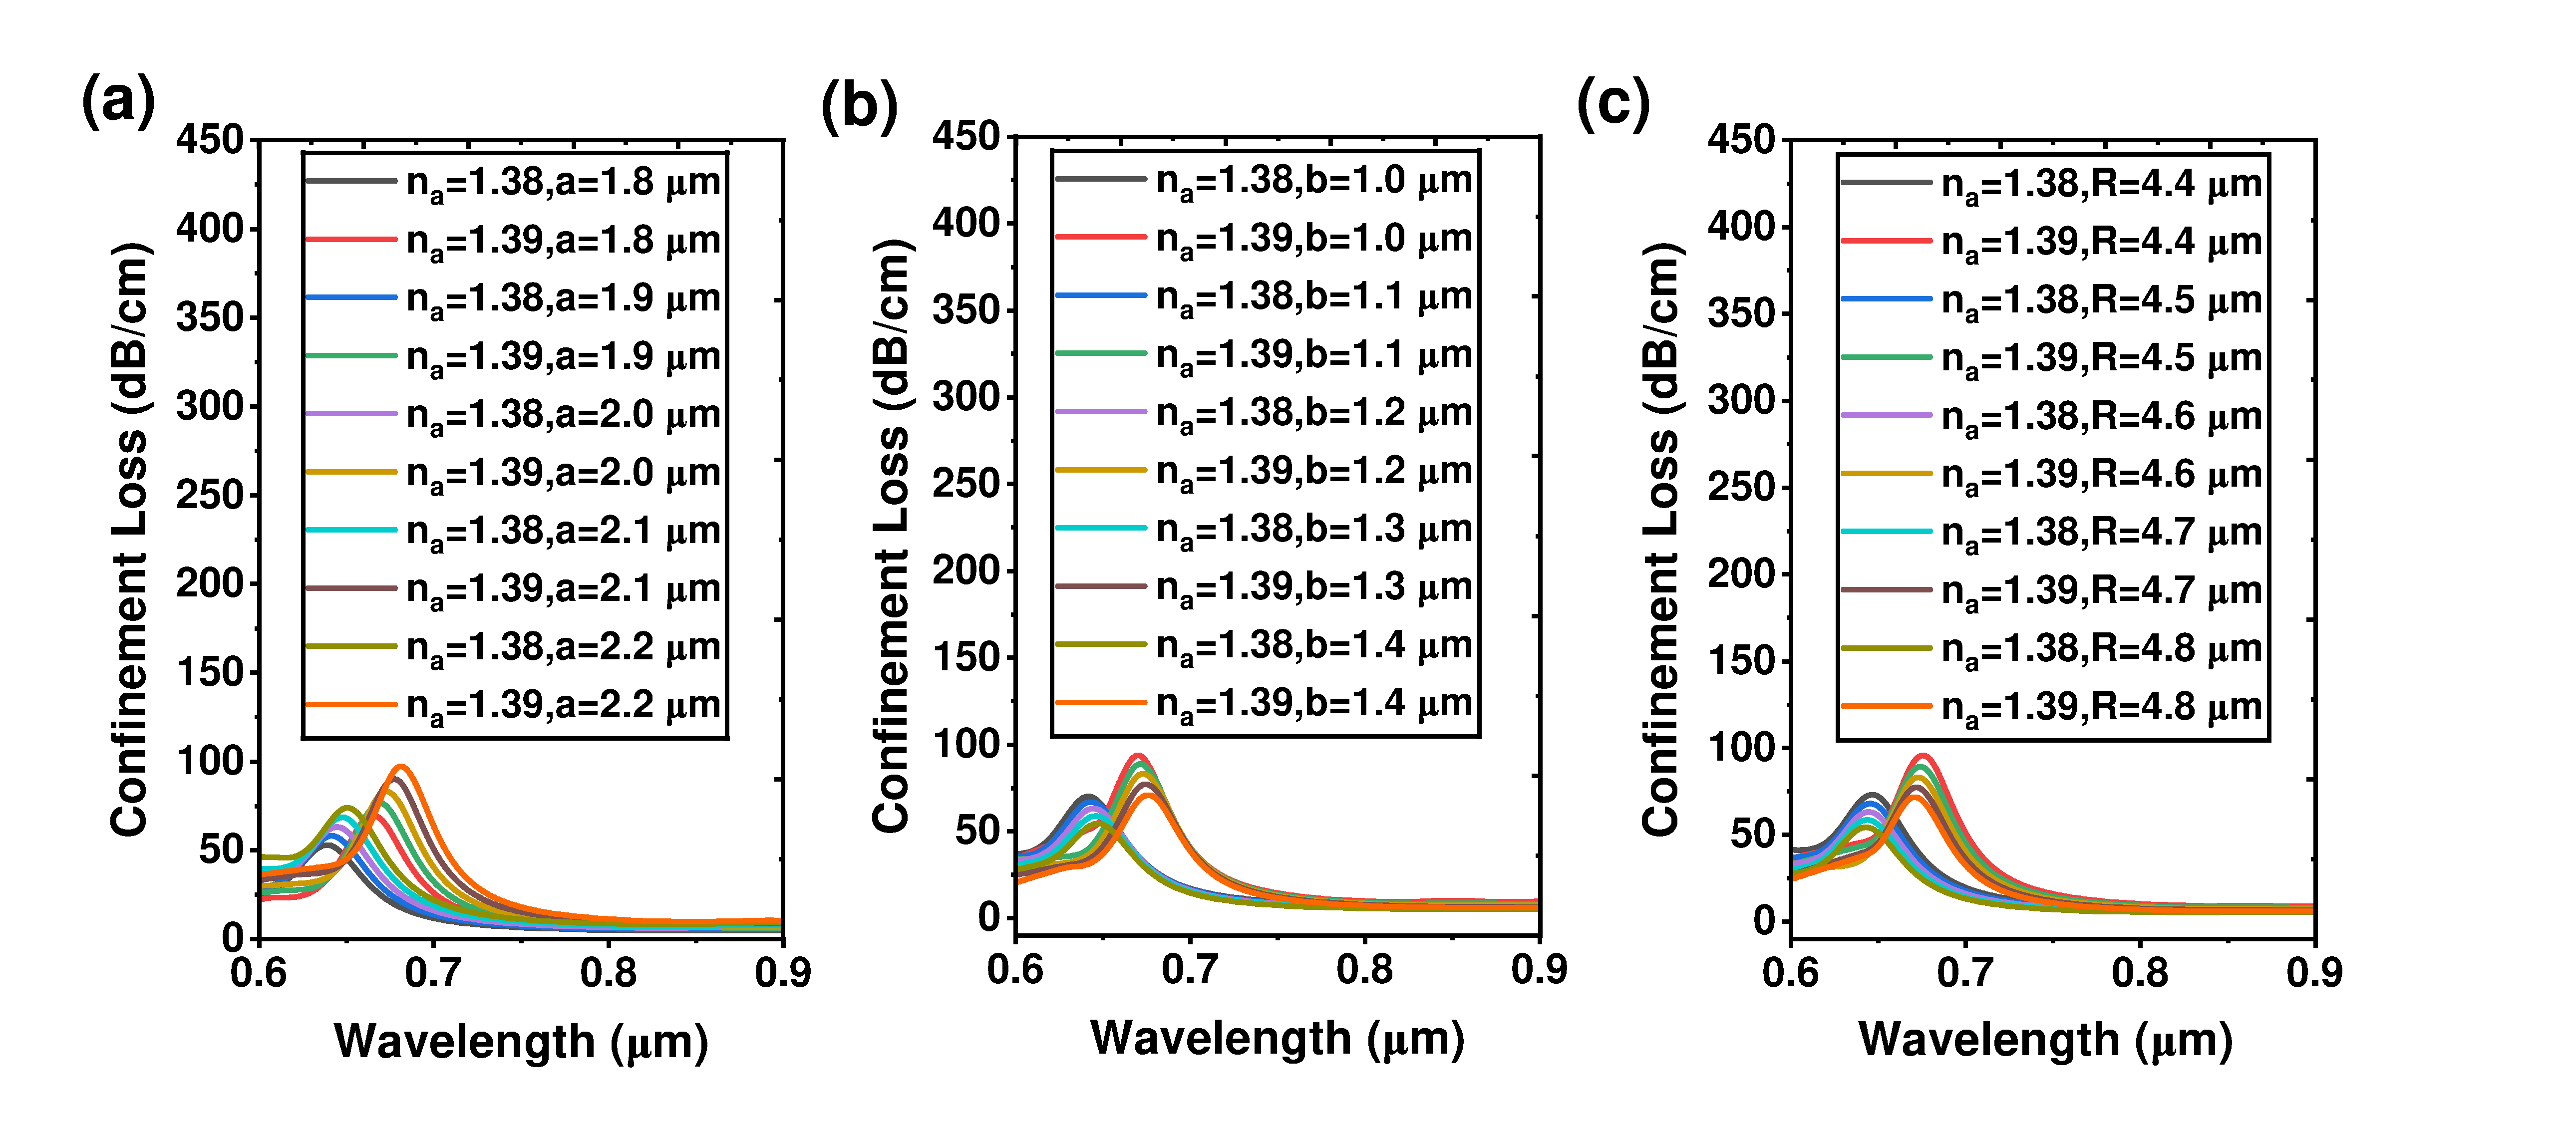
\includegraphics[width=\columnwidth]{ABR2S-1.pdf}

\vspace{0.3cm}

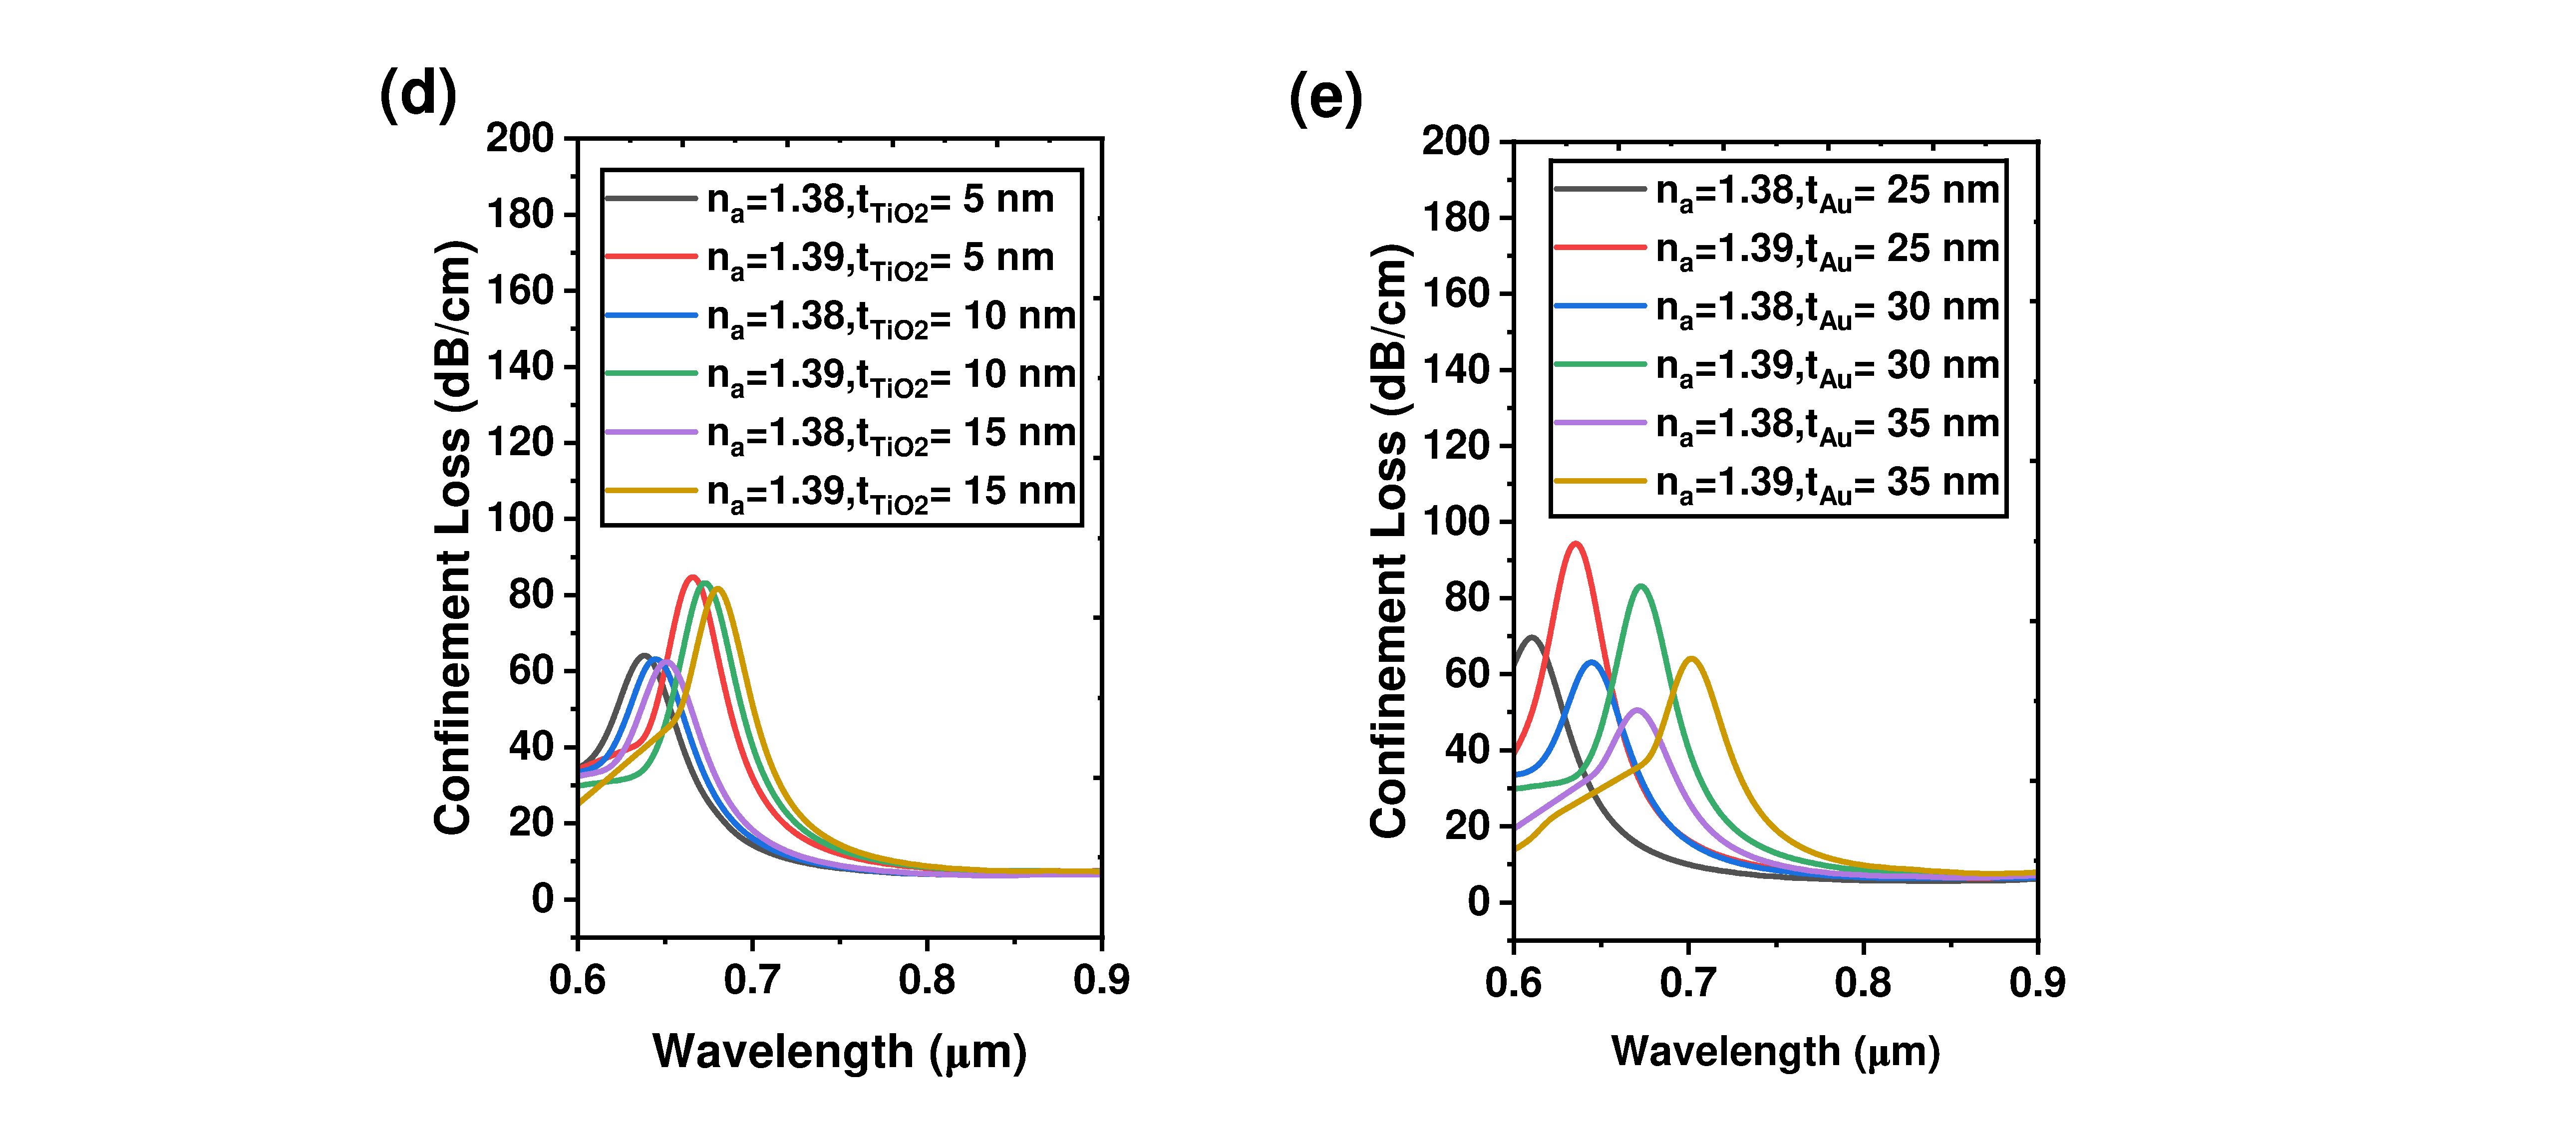
\includegraphics[width=\columnwidth]{TiO2,Au_St.pdf}

\caption{Effect of (a) semi-major axis $a$, (b) semi-minor axis $b$, (c) radial distance $R$, (d) TiO$_2$ thickness, and (e) Au thickness on the confinement-loss spectra at RI = 1.38 and 1.39.}
\label{fig:optimization_curves}
\end{figure}
The selected parameter set is $a=2.0~\mu\mathrm{m}$, $b=1.2~\mu\mathrm{m}$, $R=4.6~\mu\mathrm{m}$, $t_{\mathrm{TiO_2}}=10$~nm, and $t_{\mathrm{Au}}=30$~nm. This combination maintains suitable light confinement while preserving strong interaction with the plasmonic layer, giving a balanced overall sensing response.

\subsection{Optimization of Semi-Major Axis Parameter ($a$)}
The influence of the semi-major axis is studied by changing $a$ from $1.8$ to $2.2~\mu\mathrm{m}$, as presented in Fig.~\ref{fig:optimization_curves}(a). Every tested value gives 3000~nm/RIU wavelength sensitivity. The peak CL at $n_a=1.38$ increases from 55.61 to 77.41~dB/cm across this range, while at $n_a=1.39$ it rises from 70.43 to 100.29~dB/cm. The larger dimensions strengthen loss but can make it excessive, whereas the smaller dimensions produce a weaker amplitude response. The value $a=2.0~\mu\mathrm{m}$ is therefore selected because it keeps the resonance positions at $0.64$ and $0.67~\mu\mathrm{m}$, gives peak-loss values of 64.15 and 87.06~dB/cm, and maintains 3000~nm/RIU wavelength sensitivity with $-213.36~\mathrm{RIU}^{-1}$ amplitude sensitivity.
\begin{table*}[!t]
\centering
\caption{Parameter sweep and selected dimensions of the proposed TiO$_2$-Au-coated U-slotted elliptical-air-hole PCF-SPR sensor.}
\label{tab:optimization_results}

\renewcommand{\arraystretch}{1.25}
\setlength{\tabcolsep}{4pt}
\scriptsize
\normalfont

\begin{tabular*}{\textwidth}{@{\extracolsep{\fill}}
l c c c c c c c
@{}}

\toprule

\textbf{Parameter}
& \textbf{Value}
& \multicolumn{2}{c}{\textbf{$\lambda_{\mathrm{peak}}$ ($\mu$m)}}
& \multicolumn{2}{c}{\textbf{Peak CL (dB/cm)}}
& \textbf{$S_{\lambda}$}
& \textbf{$S_A$}
\\

\cmidrule(lr){3-4}
\cmidrule(lr){5-6}

&
& \textbf{$n_a=1.38$}
& \textbf{$n_a=1.39$}
& \textbf{$n_a=1.38$}
& \textbf{$n_a=1.39$}
& \textbf{(nm/RIU)}
& \textbf{(RIU$^{-1}$)}
\\

\midrule

\multirow{5}{*}{$a$ ($\mu$m)}
& 1.8 & 0.64 & 0.67 & 55.61 & 70.43 & 3000 & -193.92 \\
& 1.9 & 0.64 & 0.67 & 60.72 & 81.25 & 3000 & -203.00 \\
& \textbf{2.0} & 0.64 & 0.67 & 64.15 & 87.06 & 3000 & -213.36 \\
& 2.1 & 0.65 & 0.68 & 71.25 & 94.27 & 3000 & -210.63 \\
& 2.2 & 0.65 & 0.68 & 77.41 & 100.29 & 3000 & -224.48 \\

\midrule

\multirow{5}{*}{$b$ ($\mu$m)}
& 1.0 & 0.64 & 0.67 & 73.37 & 100.04 & 3000 & -210.86 \\
& 1.1 & 0.64 & 0.67 & 69.00 & 94.31 & 3000 & -212.93 \\
& \textbf{1.2} & 0.64 & 0.67 & 64.15 & 87.06 & 3000 & -213.36 \\
& 1.3 & 0.65 & 0.67 & 60.24 & 78.87 & 2000 & -211.38 \\
& 1.4 & 0.65 & 0.68 & 56.33 & 72.83 & 3000 & -207.19 \\

\midrule

\multirow{5}{*}{$R$ ($\mu$m)}
& 4.4 & 0.65 & 0.68 & 75.23 & 97.68 & 3000 & -211.22 \\
& 4.5 & 0.65 & 0.67 & 69.10 & 91.91 & 2000 & -213.10 \\
& \textbf{4.6} & 0.64 & 0.67 & 64.15 & 87.06 & 3000 & -213.36 \\
& 4.7 & 0.64 & 0.67 & 60.14 & 81.77 & 3000 & -212.66 \\
& 4.8 & 0.64 & 0.67 & 56.19 & 76.29 & 3000 & -211.39 \\

\midrule

\multirow{3}{*}{$t_{\mathrm{TiO_2}}$ (nm)}
& 5  & 0.64 & 0.67 & 66.80 & 86.69 & 3000 & -204.35 \\
& \textbf{10} & 0.64 & 0.67 & 64.15 & 87.06 & 3000 & -213.36 \\
& 15 & 0.65 & 0.68 & 65.45 & 86.75 & 3000 & -213.67 \\

\midrule

\multirow{3}{*}{$t_{\mathrm{Au}}$ (nm)}
& 25 & 0.61 & 0.64 & 72.93 & 96.12 & 3000 & -188.13 \\
& \textbf{30} & 0.64 & 0.67 & 64.15 & 87.06 & 3000 & -213.36 \\
& 35 & 0.67 & 0.70 & 52.73 & 67.29 & 3000 & -203.58 \\

\bottomrule

\end{tabular*}
\end{table*}

\subsection{Optimization of Semi-Minor Axis Parameter ($b$)}

The semi-minor axis $b$ is varied from $1.0$ to $1.4~\mu\mathrm{m}$, as shown in Fig.~\ref{fig:optimization_curves}(b). The resonance position changes only slightly, while the peak confinement loss decreases as $b$ increases. For $n_a=1.38$, the loss falls from 73.37 to 56.33~dB/cm, and for $n_a=1.39$, it decreases from 100.04 to 72.83~dB/cm. Although smaller values of $b$ produce higher loss peaks, their amplitude sensitivity is lower, while $b=1.3~\mu\mathrm{m}$ reduces the wavelength sensitivity to 2000~nm/RIU. Therefore, $b=1.2~\mu\mathrm{m}$ is selected, giving resonance wavelengths of $0.64$ and $0.67~\mu\mathrm{m}$, peak losses of 64.15 and 87.06~dB/cm, wavelength sensitivity of 3000~nm/RIU, and amplitude sensitivity of $-213.36~\mathrm{RIU}^{-1}$.

\subsection{Optimization of Radial Distance ($R$)}

The radial distance $R$ controls the position of the elliptical holes relative to the core and affects both light confinement and core-SPP coupling. In Fig.~\ref{fig:optimization_curves}(c), $R$ is varied from $4.4$ to $4.8~\mu\mathrm{m}$. Most values provide a wavelength sensitivity of 3000~nm/RIU, whereas $R=4.5~\mu\mathrm{m}$ gives only 2000~nm/RIU. Smaller values produce unnecessarily high confinement loss, while larger values slightly reduce the amplitude response. Thus, $R=4.6~\mu\mathrm{m}$ is chosen as the best trade-off, with resonance wavelengths of $0.64$ and $0.67~\mu\mathrm{m}$, peak losses of 64.15 and 87.06~dB/cm, wavelength sensitivity of 3000~nm/RIU, and amplitude sensitivity of $-213.36~\mathrm{RIU}^{-1}$.

\subsection{Optimization of TiO$_2$ Layer Thickness}

The TiO$_2$ thickness is tested at 5, 10, and 15~nm to study its effect on guided-mode and plasmonic-mode coupling. All three values provide a wavelength sensitivity of 3000~nm/RIU. The 5~nm layer gives the weakest amplitude response, while increasing the thickness from 10 to 15~nm offers only a minor improvement. Therefore, 10~nm is selected, producing resonance wavelengths of $0.64$ and $0.67~\mu\mathrm{m}$, peak losses of 64.15 and 87.06~dB/cm, and amplitude sensitivity of $-213.36~\mathrm{RIU}^{-1}$.

\subsection{Optimization of Au Layer Thickness}

The Au thickness is varied from 25 to 35~nm to examine its effect on SPP excitation and modal coupling. All tested values maintain a wavelength sensitivity of 3000~nm/RIU. The 25~nm layer gives lower amplitude sensitivity, while the 35~nm layer shifts the resonance to longer wavelengths but reduces both peak loss and amplitude response. Hence, 30~nm is selected, giving resonance wavelengths of $0.64$ and $0.67~\mu\mathrm{m}$, peak losses of 64.15 and 87.06~dB/cm, and the highest amplitude sensitivity of $-213.36~\mathrm{RIU}^{-1}$.




\section{Conclusion}

A machine-learning-assisted TiO$_2$-Au-coated U-slotted elliptical-air-hole PCF-SPR sensor is developed for RI sensing. The design uses five elliptical holes, including a U-shaped analyte channel that strengthens field interaction at the plasmonic surface. FEM simulations cover RI values of 1.33-1.44 and wavelengths of $0.4$-$1.6$~\textmu m, with the resonance shifting from $0.56$ to $1.39$~\textmu m. The optimized sensor achieves a maximum wavelength sensitivity of 44,000~nm/RIU, amplitude sensitivity of $-1167.11$~RIU$^{-1}$, FOM of 1100~RIU$^{-1}$, and minimum resolution of $2.27\times10^{-6}$~RIU.Distinct resonance peaks for normal, HeLa, and MCF-7 cell RI values show that the sensor can distinguish normal and cancer-associated samples. The peak-aligned GPR model reproduces the FEM spectra with $R^2=0.99729$, reducing the need for repeated simulations. Compared with selected ML-assisted SPR sensors, the proposed design offers a higher reported maximum wavelength sensitivity and shows potential for RI measurement, cancer-cell analysis, chemical sensing, and environmental monitoring.

\bibliography{wileyNJD-ACS}

\end{document}
